\documentclass[10pt,english]{article}

\usepackage{geometry}
\geometry{verbose,letterpaper,tmargin=1in,bmargin=1in,lmargin=1in,rmargin=
1in}
\usepackage{helvet}
\usepackage[T1]{fontenc}
\usepackage[latin1]{inputenc}
\usepackage{setspace}
\usepackage{paralist}
\usepackage{color}
\usepackage{hyperref}
 \hypersetup{backref,colorlinks=true}
\usepackage{ae,aecompl}
\usepackage{graphicx}
\usepackage{picins}
\usepackage{fancyhdr}
\usepackage{extramarks}
\usepackage{makeidx}
\pagestyle{empty}
%define tip float
\usepackage{float}
\floatstyle{ruled}
\newfloat{Tip}{H}{lox}
\floatname{Tip}{Tip}
\newcommand\qgistip[1]{\raggedright\small{#1}}
\renewcommand{\topfraction}{0.85}
 \renewcommand{\textfraction}{0.1}
\renewcommand{\floatpagefraction}{0.75}
\makeindex
%\renewcommand\familydefault{lucidabrightsans}
\title{Quantum GIS User Guide\\
\large Version 0.6 \textsl{'Simon'}}
\author{Gary E. Sherman \\Tim Sutton \\Radim Blazek (GRASS)}
%\date{\small July 2004}

\begin{document}


% To disable first line indents of paragraphs after the first one
\setlength{\parindent}{0in}


\maketitle
\tableofcontents
\listof{Tip}{QGIS Tips}
%\newpage

%\fancyfoot[C]{\thepage}
\pagestyle{fancy}
\fancyhead[L]{QGIS User Guide}
\fancyhead[R]{\textsl{Version 0.6}}


\begin{onehalfspace}
\reversemarginpar
\section{Introduction}
Quantum GIS (QGIS) is designed to be a Geographic Information System
(GIS) built for Linux/Unix, Mac OSX, and Windows. QGIS currently offers basic support for
vector (both disk-based and database) and raster formats. 

QGIS is released under the GNU Public License. You should have received a full copy of the license with your copy of QGIS.
\begin{quote}
\begin{singlespace}
\textsl{Note - The latest version of this document can always be found at\\
http://qgis.sourceforge.net/docs/userguide.html }
\end{singlespace}
\end{quote}
\section{Whats New in 0.6}
New features in version 0.6 include:
\begin{compactenum}
\item GEOS support in the OGR provider to refine selection of features via identify. This improves over the previous method of feature selection which used a simple MBR intersection check.
\item PostGIS editing support in provider
\item Vector dialog redesign to improve usability
\item Improvement in project handling (loading and saving)
\item Scale dependent rendering
\item User option to load layers with out drawing them, thus allowing you to set scale dependency, etc without waiting for the initial draw to complete
\item Interrupt drawing of features by hitting ESC
\item Attribute actions - the ability to run an external program based on the contents of an attribute field in a layer
\item Create new vector layer (shapefile) for editing
\item Windows installer
 Mac OSX binary
\item New options in the graticule builder plugin
\item Enhancements to the GPS plugin
\item Man page
\item Save delimited text as shapefile
\item Improved Delimited Text plugin, including preview of text file
\item Improved SPIT handling of PostgreSQL reserved words and shapefiles with multiple geometry types
\item Display SQL query used to create a PostGIS layer
\item PostgreSQL query builder
\item Ability to redefine the query used for PostgreSQL layers from the layer properties dialog
\item North arrow, scalebar, and copyright plugins save their state in the project file
\item Datasets with UTF8, Kanjii and CJK filenames now load properly

\end{compactenum}
\section{Major Features}

QGIS has many common GIS features and functions. The major features
are listed below. 

\begin{compactenum}
\item Support for spatially enabled PostgreSQL tables using PostGIS 
\item Support for ESRI shapefiles and other vector formats support by the
OGR library, including MapInfo files 
\item Identify features 
\item Display attribute table 
\item Select features 
\item Label features
\item Persistent selections 
\item Save and restore projects
\item Support for raster formats supported by the GDAL library 
\item Change vector symbology (single, graduated, unique value, and continuous) 
\item SVG markers symbology (single, unique value, and graduated) 
\item Display raster data such as digital elevation models, aerial photography
or landsat imagery 
\item Change raster symbology (grayscale, pseudocolor and multiband RGB) 
\item Export to Mapserver map file 
\item Preliminary digitizing support
\item Map overview
\item Plugins 
\end{compactenum}

\section{Getting Started}

This section gives you a quick overview of running QGIS and examining
data available on the QGIS web page.


\subsection{Installation}
\index{installation}
Installation of QGIS is documented in the Installation Guide. The Installation Guide is distributed with the QGIS source code and is also available at \url{http://qgis.org}.


\subsection{Sample Data}
\index{data!sample}
If you do not have any GIS data handy, you can obtain a dataset for Alaska from the QGIS web site at \url{http://qgis.org}. The Alaska data set will be used as the basis for the examples and screenshots provided in this document.


\subsection{Starting QGIS}

Assuming that QGIS is installed in the PATH, you can start QGIS by
typing: \textbf{qgis}  at a command prompt or by double clicking on the QGIS application link (or shortcut) on the desktop.
%\begin{figure}
%\caption{QGIS Main Window}
%\end{figure} 
\subsubsection{Command Line Options}\index{command line options}
QGIS supports a number of options when started from the command line. To get a
list of the options, enter \texttt{qgis ---help} on the command line. The usage
statement for QGIS is:
\small
\begin{verbatim}
Usage: /home/gsherman/qgis06_rc/bin/qgis [options] [FILES]
  options:
        [--snapshot filename]   emit snapshot of loaded datasets to given file
        [--lang language]       use language for interface text
        [--project projectfile] load the given QGIS project
        [--help]                this text
  FILES:
    Files specified on the command line can include rasters,
    vectors, and QGIS project files (.qgs):
     1. Rasters - Supported formats include GeoTiff, DEM
        and others supported by GDAL
     2. Vectors - Supported formats include ESRI Shapefiles
        and others supported by OGR and PostgreSQL layers using
        the PostGIS extension

\end{verbatim}
\normalsize
\begin{Tip} \caption{\textsc{Example Using command line arguments}}
\qgistip{
You can start QGIS by specifying one or more data files
on the command line. For example, assuming you are in your data directory,
you could start QGIS with two shapefiles and a raster file set to
load on startup using the following command: 
\ttfamily{	qgis ak\_shade.tif alaska.shp majrivers.shp}
}
\end{Tip}

\subsection{The QGIS Main Window}\index{main window}
When QGIS starts, an empty window is displayed as shown below.

\begin{figure}[h]
   \begin{center}
   \caption{Main window}\label{fig:startup}
   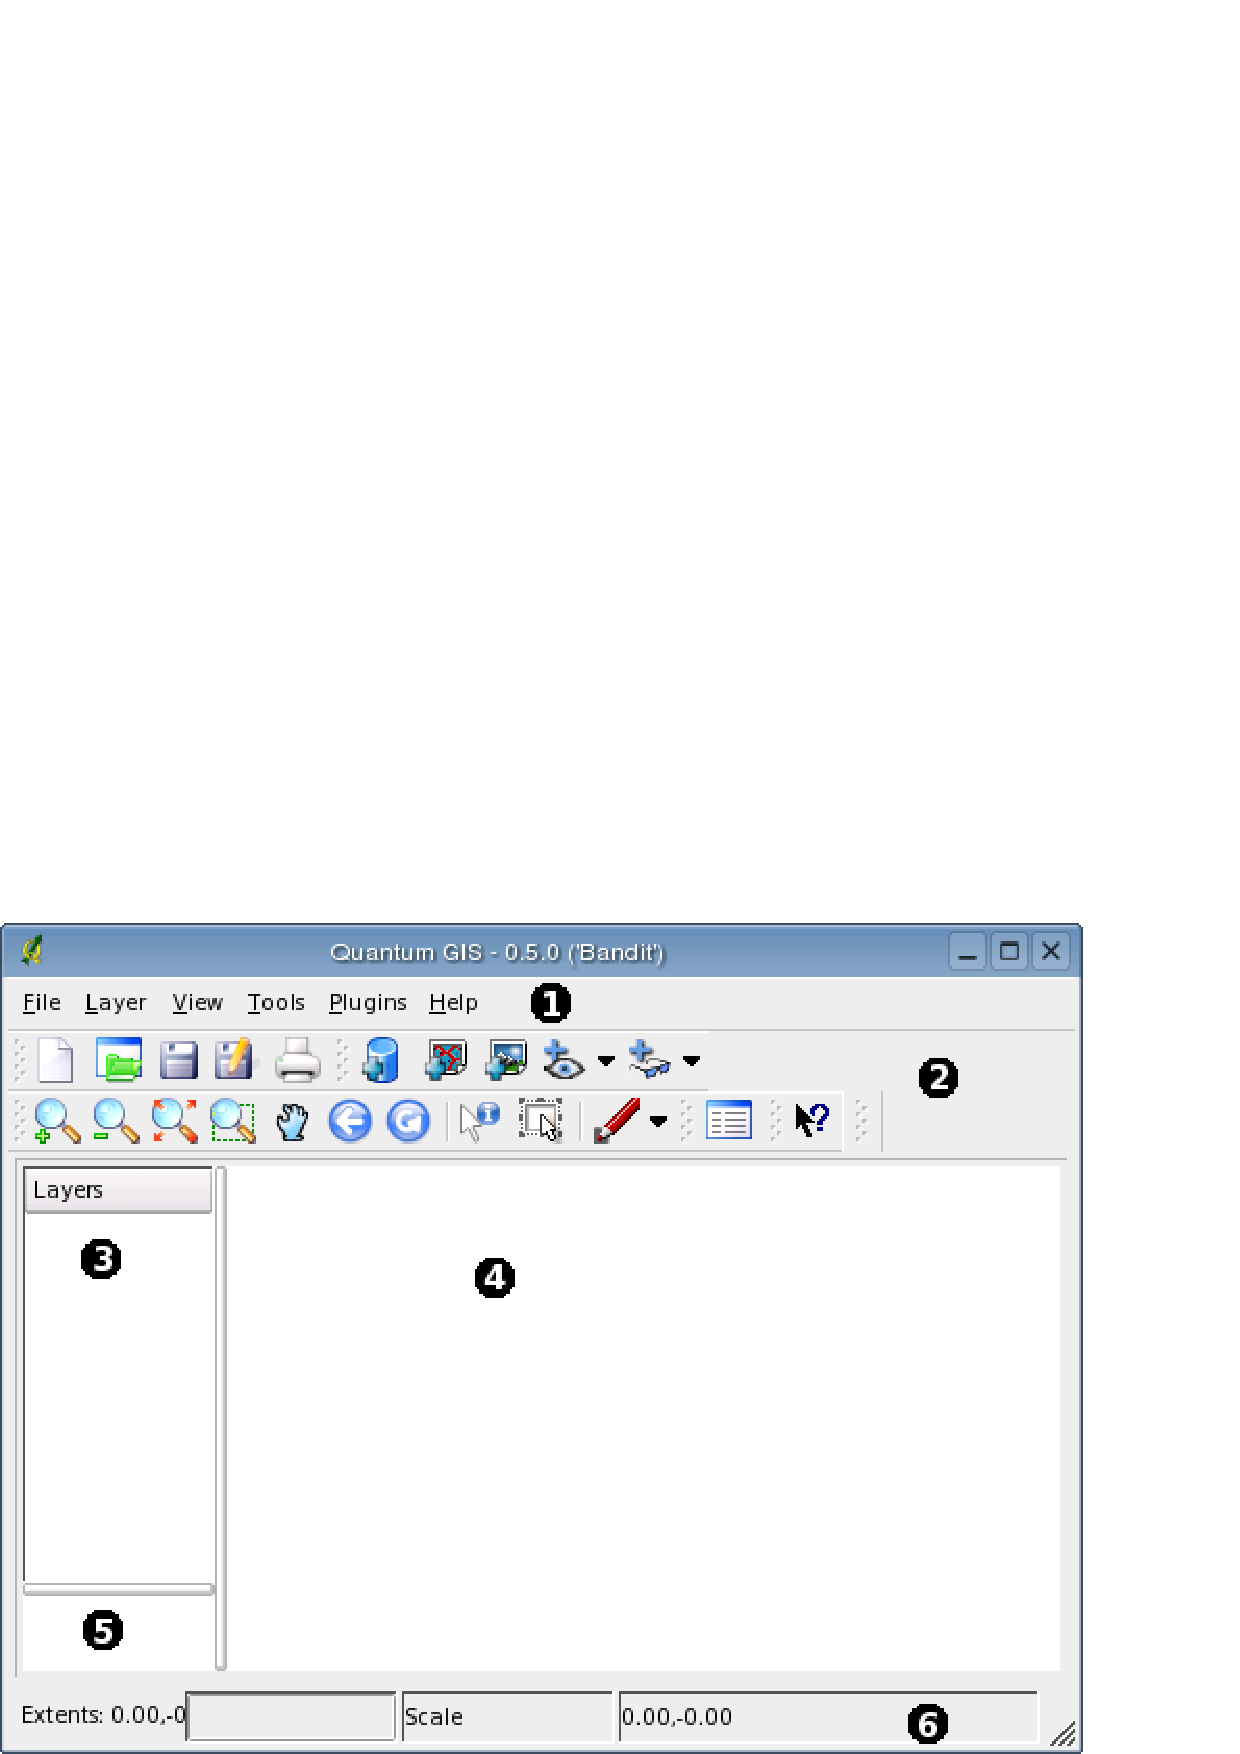
\includegraphics[scale=.9]{qgis_user_guide_images/startup}
\end{center}  
   
\end{figure}
\
textsc{Note - Your window decorations (title bar, etc.) may appear different depending on your operating system and window manager}
The QGIS main window is divided into five areas:
\begin{compactenum}
\item The menu bar
\item The tool bar
\item The map legend
\item The map view
\item The map overview
\item The status bar
\end{compactenum}

These six components of the QGIS interface are described in more detail in the following sections
\subsubsection{The QGIS menu bar}
\index{menus}
The menu bar provides access to various QGIS features using a standard windows
heirachical menu. The top-level menus and a summary of some of the functions provided are:
\begin{compactitem}
\item File (project open, save, export image, properties)
\item Layer (add, show, hide layers)
\item View (zoom, refresh)
\item Tools (plugin manager, preferences)
\item Plugins (menus added by plugins as they are loaded)
\item Help (documentation and web links)
\end{compactitem}
%See Appendix \ref{app_menu} for complete descriptions of the menu items.

\subsubsection{Toolbars}
\index{toolbars}
The toolbars provide access to most of the same functions as the menus, plus
additional tools for interacting with the map. Each toolbar item has popup
help available. Hold your mouse over the item and a short description of the
tool's purpose will be displayed. %See Appendix \ref{app_toolbar} for complete
%descriptions and illustrations of the various toolbars.  

\subsubsection{The QGIS map legend}
\index{legend}
The map legend area is used to set the visibility and z-ordering of layers.
Z-ordering means that layers listed nearer the top of the legend are drawn
over layers listed lower down in the legend. The checkbox in each legend entry
can be used to show/hide that layer.\index{layer!visibility}
\begin{Tip} \caption{\textsc{Viewing the Layer Menu}}\index{layer!context menu}
\qgistip{You can display the context menu for any layer in the legend by right-clicking
on the layer name. The context menu contains items for working with the layer and viewing
its properties.}
\end{Tip}

\subsubsection{The QGIS map view}
\index{map!view}
This is the 'business end' of QGIS - maps are displayed in this area! The map
displayed in this window will depend on the vector and raster layers you have
chosen to load (see sections that follow for more info on this). The map view
can be panned (shifting to focus of the map display to another region), zoomed
in and out, and supports various other actions as described in the toolbar
description above.  The map view and the legend are tightly bound to each
other - the maps in view reflect changes you make in the legend area.  
\begin{Tip}\caption{\textsc{Zooming the Map with the Mouse
Wheel}}\index{zoom!mouse wheel}
\qgistip{You can use the mouse wheel to zoom in and out on the map. Place the mouse cursor inside the map area and roll it forward (away from you) to zoom in and backwards (towards you) to zoom out.
}
\end{Tip}
\subsubsection{The QGIS map overview}
\index{map!overview}
The map overview area provides a full extent view of layers added to it. Within the view is a rectangle showing the current map extent. This allows you to quickly determine which area of the map you are currently viewing.

\subsubsection{The QGIS map status bar} 
The status bar shows you your current position in map coordinate (e.g. meters
or decimal degress) as the mouse pointer is moved accross the map view.

\section{Working with Vector Data}
QGIS supports vector data in a number of formats, including shapefiles,
MapInfo mif, and PostGIS\index{PostGIS} layers in a PostgreSQL database. Support for
additional data types is provided by plugins, for example delimited
text\index{delimited text}.\\

This section describes how to work with two common formats:
shapefiles\index{shapefile} and PostGIS\index{PostGIS} layers. Many of the
features available in QGIS work the same regardless of the vector data source.
This is by design and includes the identify, select, labeling, and attributes
functions.

\subsection{Shapefiles}\index{shapefile}
Shapefile support is provided by a library of functions (OGR
\url{http://www.remotesensing.org/gdal/ogr})\index{ogr}. See Appendix \ref{appdx_ogr} for a list of supported formats.\\

A shapefile actually consists of a minimum of three
files:\index{shapefile!format}
\begin{compactenum}
\item .shp file containing the feature geometries
\item .dbf file containing the attributes in dBase format
\item .shx index file
\end{compactenum}
The technical specification for the shapefile format can be found at\\
\url{http://www.esri.com/software/opengis/openpdf.html}\index{shapefile!specification}.
\subsubsection{Loading a Shapefile}
\parpic[l]{
\includegraphics{qgis_user_guide_images/addshapefile}}To load a
shapefile, start QGIS and click on the \textit{Add a vector layer} toolbar bar
button\index{shapefile!loading}. This same tool can be used to load any of the formats supported by the OGR library.

Clicking on the tool brings up a standard open file dialog (Figure \ref{fig:openshapefile}) which allows you to navigate the file system and load a shapefile (or other supported data source). 
\begin{figure}[h]
   \begin{center}
   \caption{Open OGR Data Source Dialog}\label{fig:openshapefile}\smallskip
   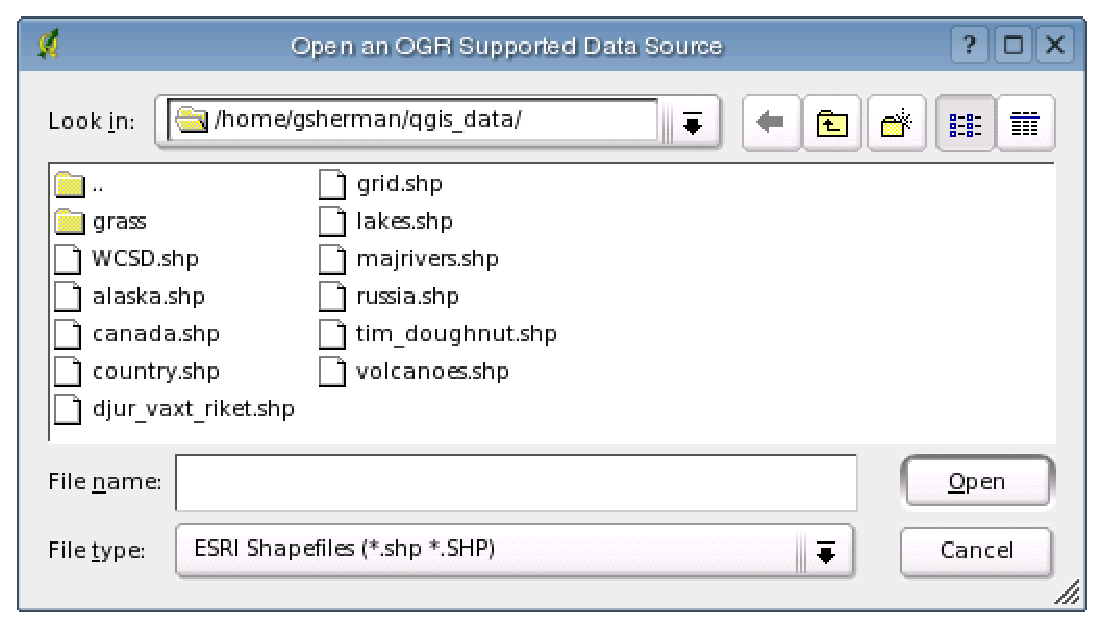
\includegraphics[scale=.75]{qgis_user_guide_images/shapefileopendialog}
\end{center}  
   
\end{figure}
Selecting a shapefile from the list and clicking Ok loads it into QGIS. Figure \ref{fig:loadedshapefile}
shows QGIS after loading the country.shp file.
\begin{figure}[h]
   \begin{center}
   \caption{QGIS with the countries Shapefile Loaded}\label{fig:loadedshapefile}\smallskip
   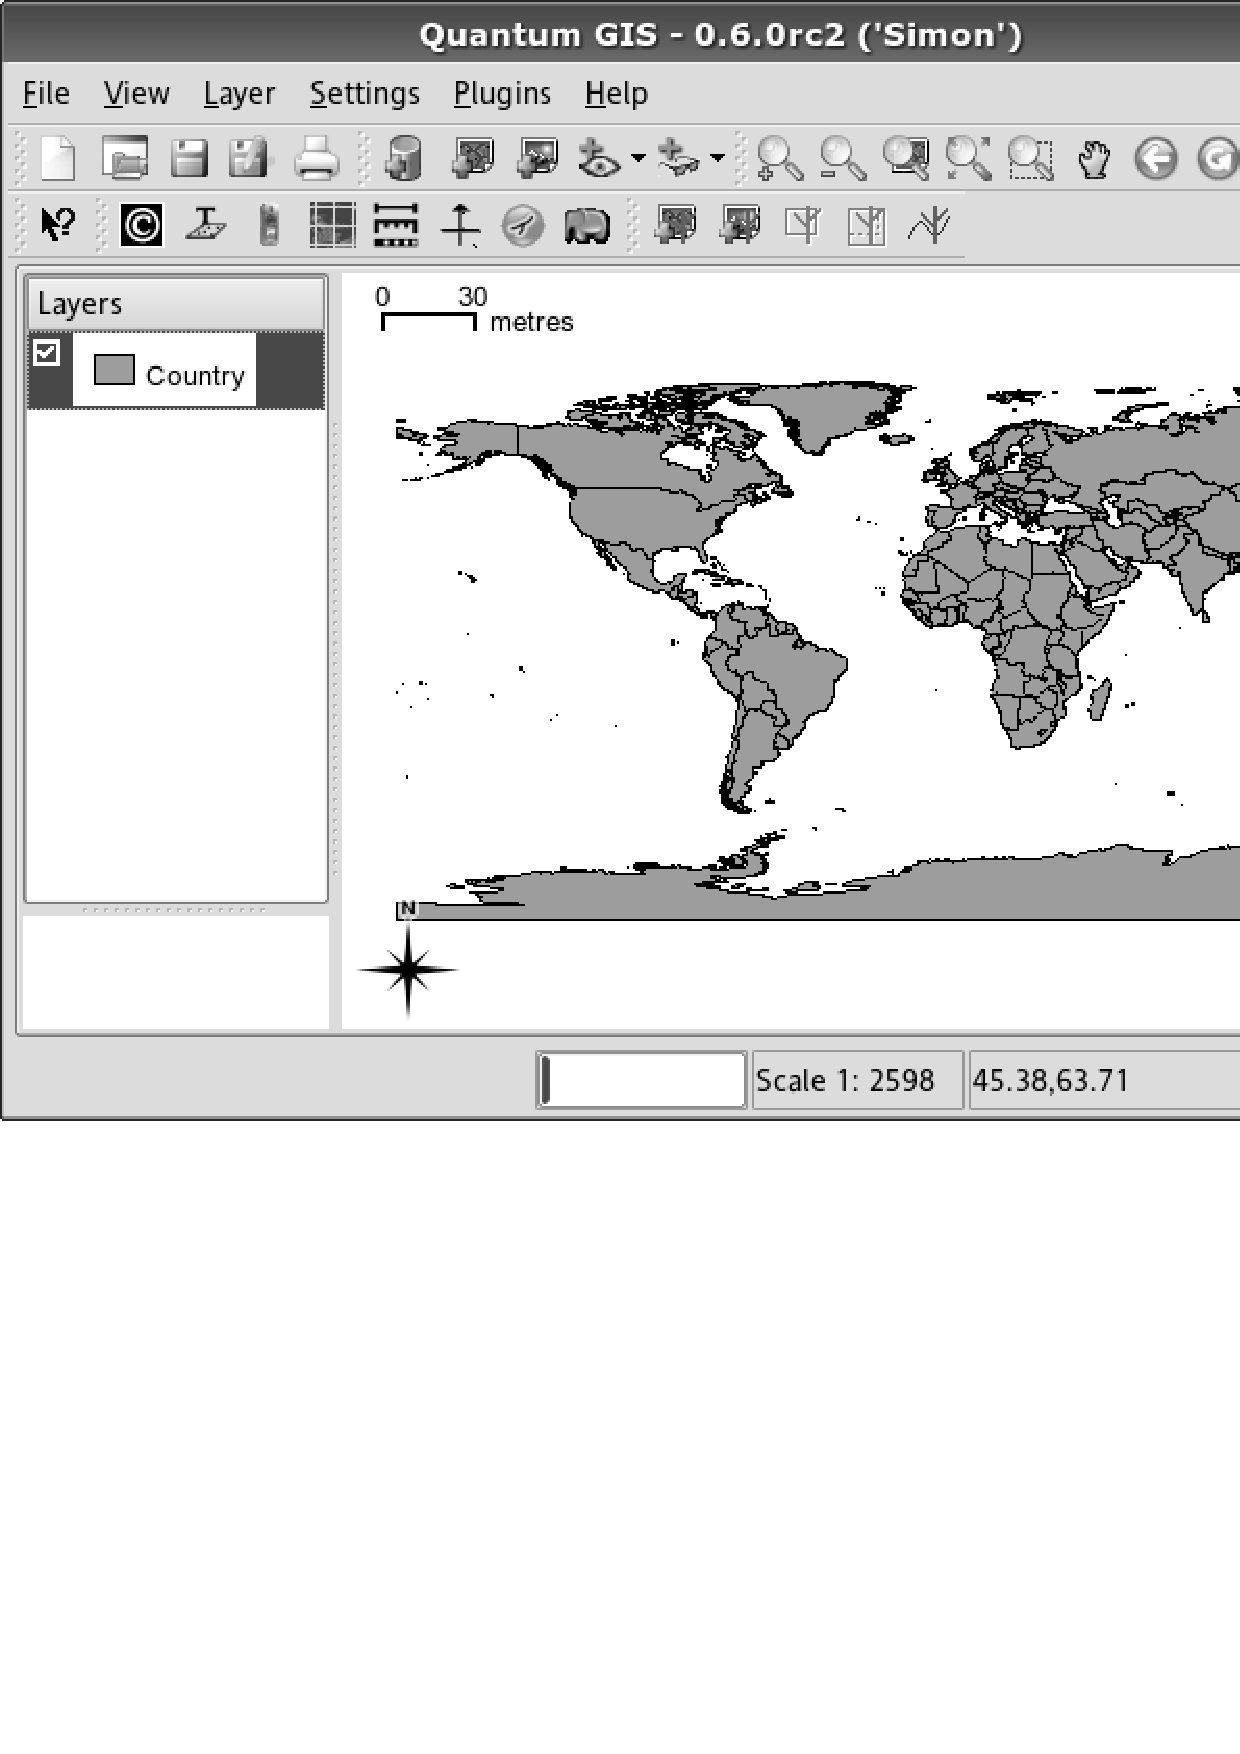
\includegraphics[scale=.6]{qgis_user_guide_images/shapefileloaded}
\end{center}  
   
\end{figure}
\begin{Tip}\caption{\textsc{Layer Colors}}
\qgistip{When you add a layer to the map, it is assigned a random color. When adding more than one layer at a time, different colors are assigned to each. }
\end{Tip}

Once loaded, you can zoom around the shapefile using the map navigation tools. To change the symbology of a layer, open the layer properties dialog by double clicking on the layer name or by right-clicking on the name in the legend and choosing \textsl{Properties} from the popup menu. See Section \ref{sec:symbology} for more information on setting symbology of vector layers.
\subsection{PostGIS Layers}\index{PostGIS!layers}
PostGIS layers are stored in a PostgreSQL database. The advantage of PostGIS is the spatial indexing, filtering, and query capability. Using PostGIS, vector functions such as select and identify work more accurately than with OGR layers in QGIS.
To use PostGIS layers you must:\index{PostgreSQL!loading layers}
\begin{compactenum}
\item Create a stored connection in QGIS to the PostgreSQL database (if one is
not already defined)\index{PostgreSQL!connection}
\item Connect to the database
\item Select the layer to add to the map
\item Optionally provide a SQL \textit{where} clause to define which features to load from the layer
\item Load the layer
\end{compactenum}
\subsubsection{Creating a Stored Connection}\index{PostgreSQL!connection}
\parpic[l]{
\includegraphics{qgis_user_guide_images/addpostgis}}The first time
you use a PostGIS data source, you must create a connection to the PostgreSQL
database that contains the data. Begin by clicking on the \textit{Add a PostGIS
Layer} toolbar button. The \textsl{Add PostGIS Table(s)} dialog will be
displayed. To access the connection manager\index{PostgreSQL!connection
manager}, click on the \textsl{New} button to
display the \textsl{Create a New PostGIS Connection} dialog. The parameters
required for a connection are shown in Table \ref{tab:postgis_connection_parms}.
\begin{table}[h]\index{PostgreSQL!connection parameters}
\centering
\caption{PostGIS Connection Parameters}\label{tab:postgis_connection_parms}\medskip
 \begin{tabular}{|l|p{5in}|}
\hline Name & A name for this connection. Can be the same as \textsl{Database}
\\
\hline Host \index{PostgreSQL!host}
& Name of the database host. This must be a resolvable host name the same as would be used to open a telnet connection or ping the host \\
\hline Database \index{PostgreSQL!database} & Name of the database  \\
\hline Port \index{PostgreSQL!port}& Port number the PostgreSQL database server listens on. The default port is 5432.\\
\hline Username \index{PostgreSQL!username}& User name used to login to the database \\
\hline Password \index{PostgreSQL!password}& password used with \textsl{Username} to connect to the database\\
\hline
\end{tabular}
\end{table}
Once the parameters have been filled in, you can test the connection by clicking
on the \textsl{Test Connection} button\index{PostgreSQL!connection!testing}. To save the password with the connection information, check the \textsl{Save Password} option.
\begin{Tip}\caption{\textsc{QGIS User Settings and
Security}}\index{settings}\index{security}
\qgistip{Your customized settings for QGIS are stored based on the operating system. On Linux/Unix, the settings are stored in your home directory in .qt/qgisrc. On Windows, the settings are stored in the registry. Depending on your computing environment, storing passwords in your QGIS settings may be a security risk.
}
\end{Tip}
\subsubsection{Loading a PostGIS Layer}\index{PostgreSQL!loading layers}
\parpic[l]{
\includegraphics{qgis_user_guide_images/addpostgis}}Once you have one or more connections defined, you can load layers from the PostgreSQL database. Of course this requires having data in PostgreSQL. See Section \ref{sec:loading_postgis_data} for a discussion on importing data into the database. \\

To load a layer from PostGIS, perform the following steps:
\begin{compactenum}
\item If the PostGIS layer dialog is not already open, click on the \textit{Add a PostGIS Layer} toolbar button
\item Choose the connection from the drop-down list and click \textsl{Connect}
\item Find the layer you wish to add in the list of available layers
\item Select it by clicking on it. You can select multiple layers by holding down the shift key while clicking. See Section \ref{sec:query_builder} for information on using the PostgreSQL Query Builder to further define the layer.
\item Click on the \textsl{Add} button to add the layer to the map
\end{compactenum}
\subsubsection{Using the Query
Builder}\label{sec:query_builder}\index{PostgreSQL!query builder}
The PostgreSQL Query Builder allows you to define a subset of a table and add it
as a layer in QGIS.  For example, if you have a towns layer with a population
field you could select only larger towns by entering \textsl{population >
100000} in the SQL box of the query builder. Figure \ref{fig:querybuilder} shows an
example of the query builder populated with data from a layer in PostgreSQL. 

\begin{figure}[h]
  \begin{center}
    \caption{PostgreSQL Query Builder}\label{fig:query_builder}\smallskip
    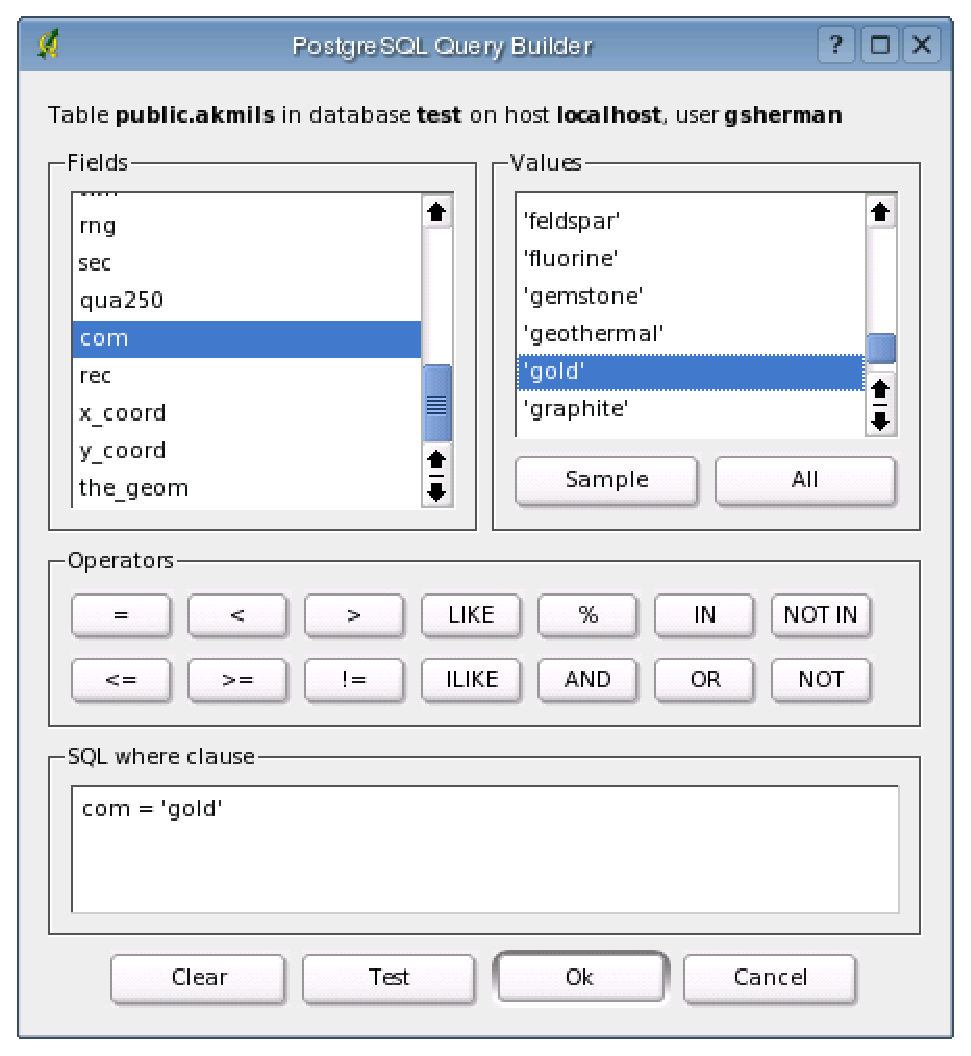
\includegraphics[scale=.6]{qgis_user_guide_images/querybuilder}
  \end{center}  
\end{figure}

The query builder\index{query builder} lists the layer's database
fields in the list box on the left.  You can get a sample of the data contained
in the highlighted field by clicking on the \textit{Sample} button\index{query
builder!generating sample list}. This
retrieves the first 25 distinct values for the field from the database. To get a
list of all possible values for a field, click on the \textit{All}
button\index{query builder!getting all values}. To
add a selected field or value to the query, double-click on it\index{query
builder!adding fields}. You can use the
various buttons to construct the query or you can just type it into the SQL box.

To test a query, click on the \textit{Test} button\index{query builder!testing
queries}. This will return a count of
the number of records that will be included in the layer. When satisfied with
the query, click \textit{Ok}. The SQL for the where clause will be shown in the
SQL column of the layer list.


\begin{Tip}\caption{\textsc{Changing the Layer Definition}}\index{query
builder!changing layer definitions}
\qgistip{You can change the layer defintion after it is loaded by altering the
SQL query used to define the layer. To do this, open the vector layer properties
dialog by double-clicking on the layer in the legend and click on the
\textit{Query Builder} button on the \textit{General} tab. See Section
\ref{sec:vectorprops} for more information.}
\end{Tip}

\subsubsection{Importing Data into PostgreSQL}\label{sec:loading_postgis_data}
\index{SPIT!importing data}
Data can be imported into PostgreSQL using a number of methods. PostGIS includes a utility called shp2pgsql that can be used to import shapefiles into a PostGIS enabled database. \\

\parpic[l]{
\includegraphics{qgis_user_guide_images/spiticon}}QGIS comes with a
plugin named SPIT (Shapefile to PostGIS Import Tool)\index{SPIT}.
SPIT can be used to load mutliple shapefiles at one time and includes support
for schemas. To use SPIT, open the Plugin Manager from the Tools menu and load
the plugin by checking the box next to the SPIT plugin and click Ok. The SPIT
icon will be added to the plugin toolbar\index{SPIT!loading}. \\

To import a shapefile, click on the SPIT tool in the toolbar to open the dialog.
You can add one or more files to the queue by clicking on the \textsl{Add}
button. To process the files, click on the Import button. The progress of the
import as well as any errors/warnings will be displayed as each shapefile is
processed.  
\begin{Tip}\caption{\textsc{Importing Shapefiles Containing
PostgreSQL Reserved Words}}\index{SPIT!reserved words}
\qgistip{If a shapefile is added to the queue containing fields that are
reserved words in the PostgreSQL database a dialog will popup showing the status
of each field. You can edit the field names\index{SPIT!editing field names}
prior to import and change any that are reserved words (or change any other
field names as desired). Attempting to
import a shapefile with reserved words as field names will likely fail.}
\end{Tip} 
\subsection{The Vector Properties
Dialog}\label{sec:vectorprops}\index{vector layers!properties dialog}
The vector properties dialog provides information about a layer, symbology
settings, and labeling options. If your vector layer has been loaded from a
PostgreSQL / Postgis datastore, you can also alter the underlying SQL for the
layer - either by hand editing the SQL on the \textit{General} tab, or by invoking the
query builder dialog on the \textit{General} tab. To access the properties dialog,
double-click on a layer in the legend or right-click on the layer and select
Properties from the popup menu.

\subsubsection{Vector Symbology}\label{sec:symbology}\index{vector
layers!symbology}

QGIS supports a number of symbology renderers to control how
vector features are displayed. Currently the following renderers
are available:

\begin{compactdesc}
    \item[Single symbol] - a single style is applied to every
    object in the layer.\index{vector layers!renderers!single symbol}
    \item[Graduated symbol] - objects within the layer are
    displayed with different symbols classified by the values of a
    particular field.\index{vector layers!renderers!graduated symbol}
    \item[Continuous colour] - objects within the layer are
    displayed with a spread of colours classified by the numerical
    values within a specified field.\index{vector layers!renderers!continous color}
    \item[Unique value] - objects are classified by the unique
    values within a specified field with each value having a
    different symbol.\index{vector layers!renderers!unique value}
\end{compactdesc}

For layers containing point features, additional renderers are
available that use SVG icons:

\begin{compactdesc}
    \item[Single marker] - a single specified icon is used for
    every point within the layer.\index{vector layers!renderers!single marker}
    \item[Graduated marker] - points within the layer are
    displayed with different icons classified by values within a
    particular field.\index{vector layers!renderers!graduated marker}
    \item[Unique value marker] - points are classified by unique
    values within a specified field with each value having a
    different icon.\index{vector layers!renderers!unique value marker}
\end{compactdesc}

To change the symbology for a layer, simply double click on its legend entry and
the vector layer properties dialog will be shown.\index{symbology!changing}

\begin{figure}[h]
   \begin{center}
   \caption{Vector Layer Properties Dialog}\label{fig:vector_symbology}\smallskip
   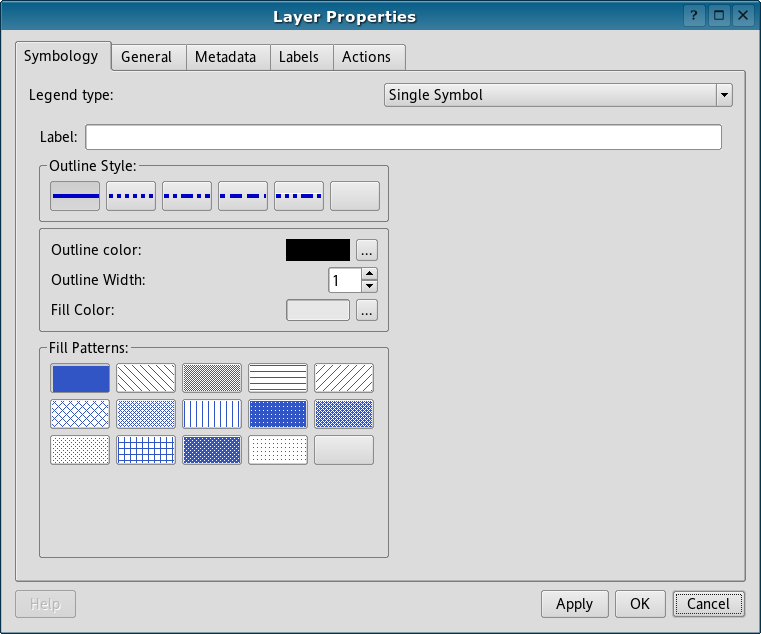
\includegraphics[scale=.5]{qgis_user_guide_images/vectorLayerSymbology}  
\end{center}  
\end{figure}
%force all figures to be printed
\clearpage

\section{Working with Raster Data}
QGIS supports a number of raster data formats. This section describes how to work with raster data in QGIS.
\subsection{What is raster data?}
index{rasters!definition}
Raster data in GIS are matrices of discrete cells that represent features on, above or below the earth's surface. Each cell in the raster grid is the same size, and cells are usually rectangular (in QGIS they will always be rectangular). Typical raster datasets include remote sensing data such as aerial photography or satellite imagery and modelled data such as an elevation matrix.\\

Unlike vector data, raster data typically do not have an associated database record for each cell.\\

In GIS, a raster layer would have georeferencing data associated with it which
will allow it to be positioned correctly in the map display to allow other
vector and raster data to be overlayed with it. QGIS makes use of georeferenced
rasters to properly display the data.\index{rasters!georeferenced}
	
\subsection{Raster formats supported in QGIS}
QGIS supports a number of different raster formats. Currently tested formats
include:\index{rasters!formats}
\begin{compactitem}
\item Arc/Info Binary Grid
\item Arc/Info ASCII Grid
\item Grass Raster
\item GeoTIFF
\item Spatial Data Transfer Standard Grids (with some limitations)
\item USGS ASCII DEM
\item Erdas Imagine
\end{compactitem}
Because the raster implmentation in QGIS is based on the GDAL library, other
raster formats implemented in GDAL are also likely to work, but have not yet
been tested. See Appendix \ref{appdx_gdal} for more
details.\index{rasters!implmentation}
	
\subsection{Loading raster data in QGIS}
\parpic[l]{
\includegraphics{qgis_user_guide_images/addraster}}Raster layers are
loaded either by clicking on the Load Raster icon or by selecting the View->Add
Raster Layer menu option. More than one layer can be loaded at the same time by
holding down the Control key and clicking on multiple items in the file
dialog.\index{rasters!loading}\\
	
\subsection{Raster Properties}

\parpic[r]{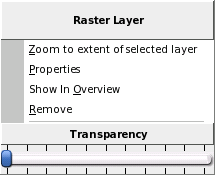
\includegraphics[scale=0.6]{qgis_user_guide_images/rastercontextmenu}}To
view and set the properties for a raster layer, right click on the layer name.
This displays the raster layer context menu that includes a number of items that
allow you to:\index{rasters!context menu}
\begin{compactitem}
\item Zoom to the full extent of the raster
\item Show the raster in the map overview window
\item Open the properties dialog (of course)
\item Remove the layer from the map
\item Set the transparency using a slider control
\end{compactitem}
Choose \textsl{Properties} from the context menu to open the raster properties
dialog for the layer.\index{rasters!properties}\\


Figure \ref{fig:raster_properties} shows the properties dialog. There are four tabs on the dialog: \textsl{Symbology}, \textsl{General}, \textsl{Metadata}, and \textsl{Pyramids}.

\begin{figure}[h]
   \begin{center}
   \caption{Raster Layers Properties Dialog}\label{fig:raster_properties}\smallskip
   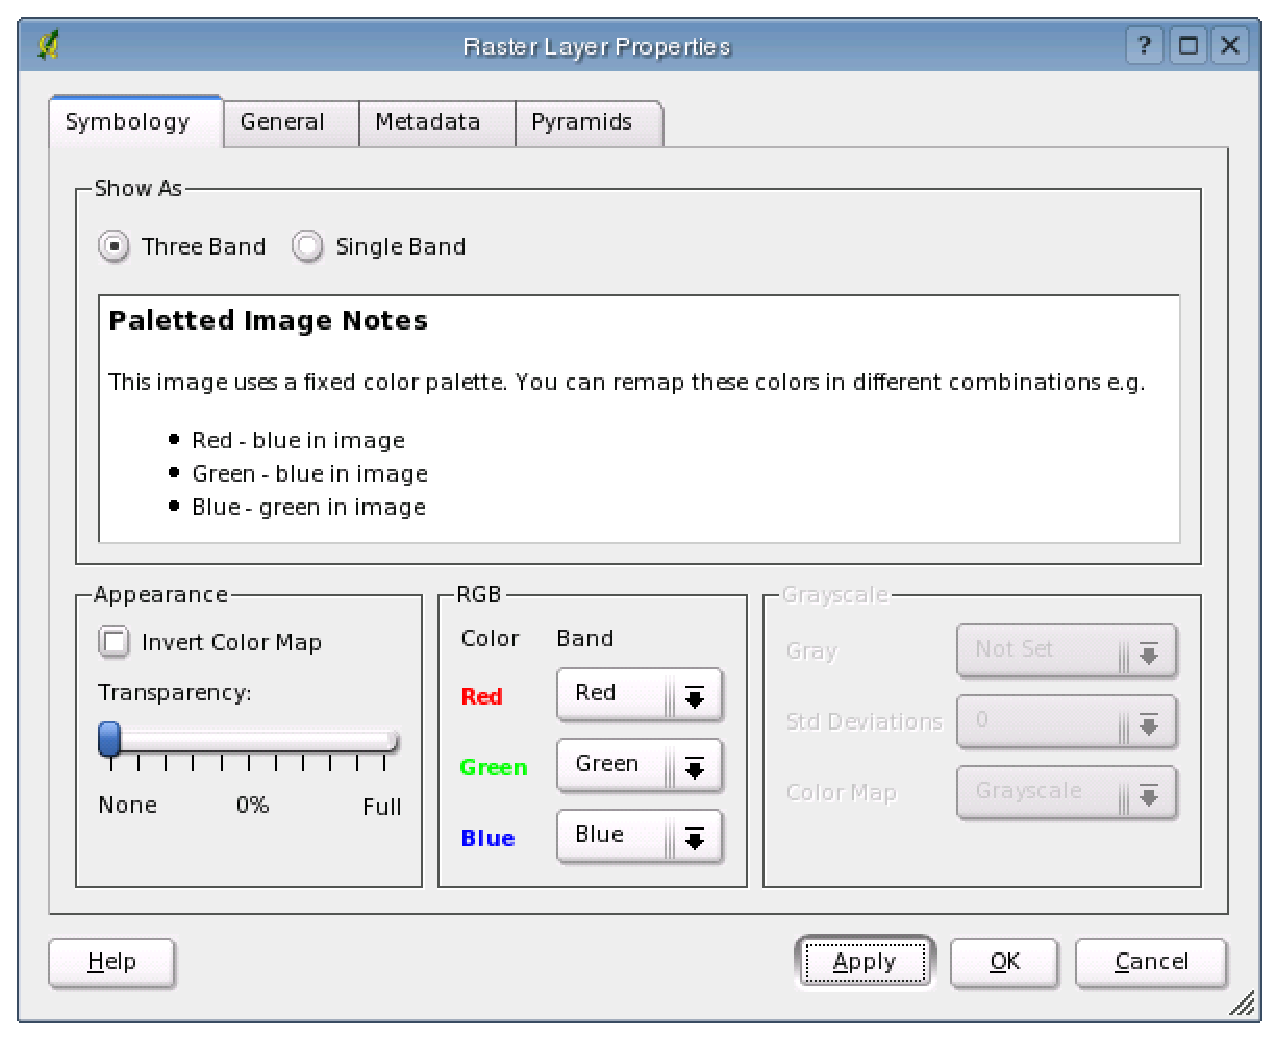
\includegraphics[scale=.7]{qgis_user_guide_images/raster_properties}
\end{center}  
\end{figure}


\subsubsection{Symbology Tab}


QGIS supports three forms of raster layers:\index{rasters!supported forms}
\begin{compactitem}
\item Single Band Grayscale Rasters
\item Palette Based RGB Rasters
\item Multiband RGB Rasters
\end{compactitem}

From these three basic layer types, eight forms of symbolised raster display can
be used:\index{rasters!renderers}
\begin{compactenum}

\item Single Band Grayscale
\item Single Band Pseudocolor
\item Paletted Grayscale (where only the red, green or blue component of the image is displayed)
\item Paletted Pseudocolor (where only the red, green or blue component of the image is displayed, but using a pseudocolor algorithm)
\item Paletted RGB
\item Multiband Grayscale (using only one of the bands to display the image)
\item Mulitiband Pseudocolor (using only one of the bands shown in pseudocolor)
\item Multiband RGB (using any combination of three bands)
\end{compactenum}
\smallskip
QGIS can invert the colors in a given layer so that light colors become dark
(and dark colors become light). Use the \textsl{Invert Color Map} checkbox to
enable / disable this behavior.\index{rasters!inverting the color map}\\

QGIS has the ability to display each raster layer at varying transparency
levels.\index{rasters!transparency} Use the transparency slider to indicate to what extent the underlying layers (if any) should be visible though the current raster layer. The transparency can also be set using the transparency slider in the layer context menu which is accessible by right-clicking on the layer in the legend.\\

QGIS can restrict the data displayed to only show cells whose values are within
a given number of standard deviations of the mean for the
layer.\index{rasters!standard deviation} This is useful when you have one or two cells with abnormally high values in a raster grid that are having a negative impact on the rendering of the raster. This option is only available for pseudocolor images.\\

\subsubsection{General Tab}
The General tab displays basic information about the selected raster, including
the layer source and  display name in the legend (which can be modified). This
tab also shows a thumbnail of the layer, its legend symbol, and the
palette.\index{rasters!properties}

\subsubsection{Metadata Tab}
The Metadata tab displays a wealth of information about the raster layer,
including statistics about each band in the current raster layer. Statistics are
gathered on a 'need to know' basis, so it may well be that a given layers
statistics have not yet been collected.\index{rasters!metadata}


\begin{Tip}\caption{\textsc{Gathering Raster Statistics}}
\qgistip{To gather statistics for a layer, select pseudocolor rendering and
click the \textsl{Apply} button. Gathering statistics for a layer can be time
consuming. Please be patient while QGIS examines your
data!\index{rasters!statistics}
}
\end{Tip}
\subsubsection{Pyramids Tab}
Large resolution raster layers can slow navigation in QGIS. By creating lower
resolution copies of the data (pyramids), performance can be considerably
improved as QGIS selects the most suitable resolution to use depending on the
level of zoom.\index{rasters!building pyramids} \\

You must have write access in the directory where the original data is stored to build pyramids. \\

Please note that building pyramids may alter the original data file and once created they cannot be removed. If you wish to preserve a 'non-pyramided' version of your raster, make a backup copy prior to building pyramids.
\section{GRASS}\label{sec:grass}\index{GRASS}
The GRASS plugin adds the following features to QGIS:
\begin{compactitem}
\item Add GRASS vector layers
\item Add GRASS raster layers
\item Vector layers digitizing
\item Changing of the GRASS region
\end{compactitem}
\subsection{Starting QGIS with
GRASS}\label{sec:starting_grass}\index{GRASS!starting QGIS}
When using the GRASS plugin, QGIS can be started in two ways: from the GRASS shell or from a regular shell.
\subsubsection{From GRASS shell}

If QGIS is started from the GRASS shell (GRASS started by grass57 command), no
additional settings are required. \index{GRASS!shell}
\subsubsection{Outside GRASS shell}

If QGIS is not started from the GRASS shell, the environment variables must be properly set before starting QGIS.\\
 
The path to GRASS libraries must be added to LD\_LIBRARY\_PATH environment
variable. For example (in bash): \index{GRASS!environment settings}
\begin{verbatim}
    export LD_LIBRARY_PATH=/usr1/grass57/dist.i686-pc-linux-gnu/lib:$LD_LIBRARY_PATH
\end{verbatim}    
 
The GISBASE environment variable must be set to the full path of the directory where GRASS is installed (the same as used for --with-grass= option). For example (in bash):
\begin{verbatim}
    export GISBASE=/usr1/grass57/dist.i686-pc-linux-gnu 
\end{verbatim}
\subsection{Loading GRASS Data}\index{GRASS!loading data}
With the GRASS plugin loaded, you can load a vector or raster layer using the appropriate button on the toolbar. \begin{Tip}\caption{\textsc{GRASS Data Loading}}
\qgistip{If you have problems loading data or QGIS terminates abnormally, check to make sure you have started GRASS properly as described in Section \ref{sec:starting_grass}.
}
\end{Tip} 
\subsection{Vector Data Model}\index{GRASS!vector data model}
It is important to understand the GRASS vector data model prior to
digitizing.\index{GRASS!digitizing}
In general, GRASS uses a topological vector model.\index{GRASS!topology} This
means that areas are not represented as closed polygons, but by one or more
boundaries. A boundary between two adjacent areas is digitized only once, and it
is shared by both areas. Boundaries must be connected without gaps. An area is
identified (labeled) by the centroid of the area.\\

Besides boundaries and centroids, a vector map can also contain
points and lines. All these geometry elements can be mixed
in one vector.\\

It is possible to store more 'layers' in one vector dataset. For example,
fields, forests and lakes can be stored in one vector. Adjacent
forest and lake can share the same boundary, but they have separate attribute tables.
It is also possible to attach attributes to boundaries. For example, the boundary between lake and forest is a road with different attribute table.\\
%In addition, one geometry element can represent a geometry for more
%features. For example, a road can be a marked turistic route at the same 
%time.

The 'layer' of the feature is defined by 'field' (sorry for this name).
'Field' is the number which defines if the geometry is forest or lake.
For now, it can be only a number, in the future GRASS will also support  
names as fields in the user interface.\\

Attributes are stored in external database tables, for example
DBF, PostgreSQL, etc.\index{GRASS!attribute storage}\\

Attributes in database tables are linked to geometry elements
using 'category'.\index{GRASS!attribute linkage} 'Category' (key, ID) is an
integer attached to geometry primitives, and it is used as the link to one
column in the database table.\\
\begin{Tip}\caption{\textsc{Learning the GRASS Vector Model}}
\qgistip{The best way to learn the GRASS vector model and its capabilities
is to download the demo mapset from \url{http://mpa.itc.it/radim/g51/g51test-12-multi.tar.gz}.
Extract the mapset, add all layers from vector 'multi' to QGIS, and query attributes.
Finaly start editing of vector 'multi', to see how those layers are stored.
}
\end{Tip} 
\subsection{Digitizing and Editing Tools}\index{GRASS!digitizing tools}
The digitizing tools for GRASS vector layers are accessed using the \textsl{Edit GRASS Vector Layer} tool on the toolbar. Make sure you have loaded a GRASS vector and it is the selected layer in the legend before clicking on the edit tool. In this release, the vector must exist prior to beginning to edit. The ability to create a new "empty" layer will be added in a future version. Figure \ref{fig:grass_edit} shows the GRASS Edit dialog that is displayed when you click on the edit tool. 
\begin{figure}[h]
   \begin{center}
   \caption{GRASS Edit Dialog}\label{fig:grass_edit}\smallskip
   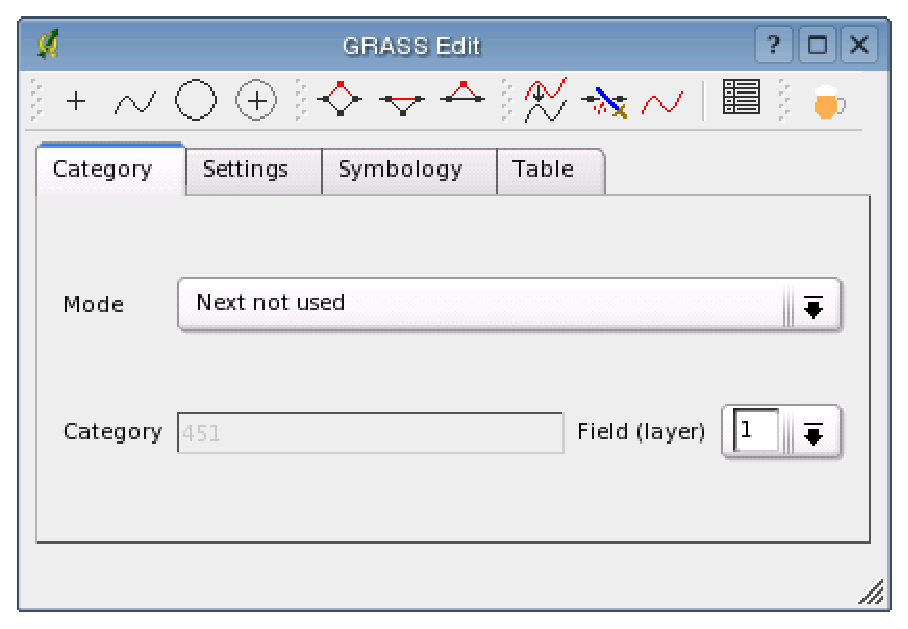
\includegraphics[scale=.7]{qgis_user_guide_images/grassedit}
\end{center}  
\end{figure}
The tools and settings are discussed in the following sections.\\
\subsubsection{Toolbar}
Table \ref{tab:grass_tools} lists the digitizing tools provided by the GRASS plugin. These correspond to the tool buttons in the toolbar(s) across the top of the dialog.
\begin{table}[h]\index{GRASS!digitizing tools}

\centering
\caption{GRASS Digitizing Tools}\label{tab:grass_tools}\medskip
 \begin{tabular}{|l|p{5in}|}
 \hline \textbf{Tool} & \textbf{Purpose} \\
\hline New Point & digitize new point \\
\hline New Line &  digitize new line (finish by selecting new tool) \\
\hline New Boundary & digitize new boundary (finish by selecting new tool)\\
\hline New Centroid & digitize new centroid (label existing area)\\
\hline Move vertex & select one vertex of existing line or boundary and identify new position\\
\hline Add vertex & add a new vertex to existing line\\
\hline Delete vertex & delete one vertex from existing line (confirm selected vertex by another click)\\
\hline Move line & select existing line and click on new position\\
\hline Split line & split an existing line to 2 parts\\
\hline Delete line & delete existing line (confirm selected line by another click)\\
\hline Edit attributes & edit attributes of existing element (note that one element can represent more features, see above)\\
\hline Mug & close digitizing session\\
\hline
\end{tabular}
\end{table}
\subsubsection{Category Tab}\index{GRASS!category settings}
This tab allows you to set the way in which the category will be assigned to each new feature and/or assign a category to a feature.
\begin{compactitem}
\item Mode: what category should be attached to geometry
\begin{compactitem}
\item Next not used - next category not yet used in vector
\item Manual entry - define the category in 'Category entry'
\item No category - digitize geometry without category
\end{compactitem}
\item Category - a number (ID) attached to digitized feature
\item Field - feature (attribute table) identification
\end{compactitem}
\subsubsection{Settings Tab} \index{GRASS!snapping tolerance}
This tab allow you to set the snapping in screen pixels. This is the threshold in pixels in which new points or line ends are snapped to existing nodes. This helps prevent gaps or dangles between boundaries

\subsubsection{Symbology Tab}\index{GRASS!symbology settings}
This tab allows you to view and set symbology for various geometry types and their topological status (e.g. closed / opened boundary).

\subsubsection{Table} \index{GRASS!table editing}
This tab provides the means to view, create, or modify the database table for a given field.
\begin{Tip}\caption{\textsc{GRASS Edit Permissions}}\index{GRASS!edit permissions}
\qgistip{You must be the owner of the GRASS mapset you want to edit. It is impossible to edit vectors in mapsets which are not yours, even if you have write permissions.
}
\end{Tip} 

\subsubsection{Region Tool}\index{GRASS!region}

The current region (window) in GRASS is very important for all 
raster modules. All new created rasters have the extension and resolution
of the current region, regardless their original region. 
The region is stored in \$LOCATION/\$MAPSET/WIND file, and it defines
north, south, east, west, number of columns, number of rows, 
horizontal and vertical resolution.\\

It is possible to switch on/off the grass region in QGIS canvas
using the \textsl{Display Current GRASS Region}
button.\\index{GRASS!region!display}\

With the \textsl{Edit Current GRASS Region} you can open a tool 
in which you can change the current region and symbology
of the rectangle on the QGIS Canvas. When the tool is running,
it is also possible to select a new region interactively
on the QGIS canvas.\index{GRASS!region!editing}\\

Both tools are available only if QGIS was started from a GRASS 
shell or if the GISRC enviroment variable pointing to a
valid GISRC file was set (i.e. only if you are running 
GRASS within your mapset).

%\subsection{The GRASS Toolbar}
%The GRASS toolbar is displayed when the GRASS plugin is loaded using the Plugin Manager (see Section \ref{sec:managing_plugins}, \textsl{Managing Plugins}). Figure  shows the toolbar with each function annotated.

\section{Using Plugins}\index{plugins}
QGIS has been designed with a plugin architecture. This allows new features/functions to be added to the application. Many of the features in QGIS are actually implemented as plugins.\\

There are two types of plugins in QGIS: core and user-contributed.
\index{plugins!types}A core plugin is maintained by the QGIS development team and is part of every QGIS distribtution. A user-contributed plugin is an external plugin that is maintained by the individual author. The QGIS Community site (\url{http://community.qgis.org}) serves as the repository for user contributed plugins.

\subsection{Finding and Installing a Plugin}
When you install QGIS, all of the core plugins are included (these are described
below). \index{plugins!installing}Additional user-contributed plugins may be
available on the QGIS Community site. To see what user-contributed plugins are
available, see the plugins page on the Community site
(\url{http://community.qgis.org/plugins}).\index{plugins!user contributed}\\

Typically user-contributed plugins are distributed in source form and require compiling. For instructions on building and installing a user-contributed plugin, see the documentation included with the plugin.
\subsection{Managing Plugins}\label{sec:managing_plugins}\index{plugins!managing}
Managing plugins consists of loading or unloading them from QGIS. Loaded plugins are "remembered" when you exit the application and restored the next time you run QGIS.\\

To manage plugins, open the \textsl{Plugin Manager} from the \textsl{Tools}
menu. \index{plugins!manager}The Plugin Manager displays all the available plugins and their status (loaded or unloaded). Figure \ref{fig:pluginmanager} shows the Plugin Manager dialog.

\begin{figure}[h]
   \begin{center}
   \caption{Plugin Manager}\label{fig:pluginmanager}\smallskip
   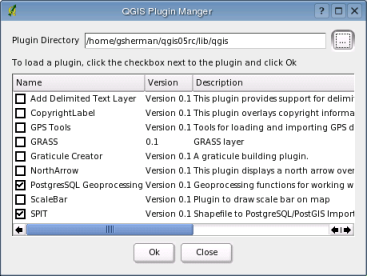
\includegraphics{qgis_user_guide_images/pluginmanager_80pct}
\end{center}  
\end{figure}
Typically all QGIS plugins are installed in the same location. This location is shown in the Plugin Directory text field. You can tell QGIS to load plugins from another location by specifying a different directory.
\begin{Tip}\caption{\textsc{Crashing Plugins}}\index{crashes}
\qgistip{If you find that QGIS crashes on startup, a plugin may be at fault. You can stop all plugins from loading by editing your .qt/qgisrc file in your home directory on Linux/Unix (Windows users will have to edit the registry). On Linux/Unix, open the qgisrc file in a text editor and find the [Plugins] section. Set all the plugin values to false to prevent them from loading. For example, to prevent the Delimited text plugin from loading, the entry in qgisrc should look like this:\ttfamily{
 Add Delimited Text Layer=false}.\normalfont  Do this for each plugin in the [Plugins] section. You can then start QGIS and add the plugins one at a time from the Plugin Manger to determine which is causing the problem.

}
\end{Tip} 

\subsection{Data Providers}\index{data providers}
Data Providers are "special" plugins that provides access to a data store. By default, QGIS supports PostGIS layers and disk-based data stores supported by the OGR library (Appendix \ref{appdx_ogr}). A Data Provider plugin extends the ability of QGIS to use other data sources.\\

Data Provider plugins are registered automatically by QGIS at startup. They are not managed by the Plugin Manager but are used behind the scenes when a corresponding data type is added as a layer in QGIS.
\subsection{Core Plugins}\index{plugins!core}
QGIS currently contains 9 core plugins that can be loaded using the Plugin Manager. Table \ref{tab:core_plugins} lists each of the core plugins along with a description of their purpose. Figure \ref{fig:plugintoolbar} shows the icon for each plugin in the Plugin toolbar (the number corresponds to the Item in Table \ref{tab:core_plugins}. Note the GRASS plugin is not included below because it installs its own toolbar (see Section \ref{sec:grass} for a discussion of available features in GRASS plugin).
\begin{table}[h]
\centering
\caption{QGIS Core Plugins}\label{tab:core_plugins}\medskip
\small
 \begin{tabular}{|l|l|p{4in}|}
\hline \textbf{Item} & \textbf{Plugin} & \textbf{Description} \\
\hline 1 & Copyright Label \index{plugins!copyright}& Display a copyright label on the map canvas\\
\hline 2 & Delimited Text \index{plugins!delimited text}& Load a delimited text file containing x,y coordinates as a point layer \\
\hline 3 & GPS Tools \index{plugins!gps}& Load and display GPS data \\
\hline 4 & Graticule Creator \index{plugins!graticule}& Create a latitude/longitude grid and save as a shapefile\\
\hline 5 & Scalebar \index{plugins!scalebar}& Add a scalebar to the map canvas\\
\hline 6 & North Arrow \index{plugins!north arrow}& Add a north arrow to the map canvas\\
\hline 7 & PostgreSQL Geoprocessing \index{plugins!geoprocessing}& Buffer a PostGIS layer \\
\hline 8 & SPIT \index{plugins!SPIT}& Shapefile to PostGIS Import Tool - import shapefiles into PostgreSQL\\
\hline
\end{tabular}
\end{table}
\normalsize
\begin{figure}[h]
   \begin{center}
   \caption{Plugin Toolbar and Icons}\label{fig:plugintoolbar}\smallskip
   
\includegraphics[scale=1.0]{qgis_user_guide_images/plugintoolbar}
\end{center}  
\end{figure}
\clearpage
\appendix
\section{Supported OGR Formats}\label{appdx_ogr} \index{ogr!supported formats}
At the date of this document, the following formats are supported by the OGR
library. Formats known to work in QGIS are indicated in \textbf{bold}.

\begin{compactitem}
\item \textbf{Arc/Info Binary Coverage}
\item Comma Separated Value (.csv) 
\item DODS/OPeNDAP
\item \textbf{ESRI Shapefile}
\item FMEObjects Gateway
\item GML
\item IHO S-57 (ENC)
\item \textbf{Mapinfo File}
\item Microstation DGN
\item OGDI Vectors
\item ODBC
\item Oracle Spatial
\item PostgreSQL\footnote{QGIS implements its own PostgreSQL functions. OGR should be built without PostgreSQL support}
\item \textbf{SDTS}
\item SQLite
\item UK .NTF
\item U.S. Census TIGER/Line
\item VRT - Virtual Datasource
\end{compactitem}
\section{GDAL Raster Formats}\label{appdx_gdal}\index{rasters!supported formats}
At the date of this document, the following formats are supported by the GDAL
library. Note that not all of these format may work in QGIS for various reasons.
For example, some require external commercial libraries. Only those formats that
have been well tested will appear in the list of file types when loading a
raster into QGIS. Other untested formats can be loaded by selecting the
\textsl{All other files (*)} filter. Formats known to work in QGIS are indicated
in \textbf{bold}.

\begin{compactitem}
\item \textbf{Arc/Info ASCII Grid}
\item \textbf{Arc/Info Binary Grid (.adf)}
\item Microsoft Windows Device Independent Bitmap (.bmp)
\item BSB Nautical Chart Format (.kap)
\item VTP Binary Terrain Format (.bt)
\item CEOS (Spot for instance)
\item First Generation USGS DOQ (.doq)
\item New Labelled USGS DOQ (.doq)
\item Military Elevation Data (.dt0, .dt1)
\item ERMapper Compressed Wavelets (.ecw)
\item ESRI .hdr Labelled
\item ENVI .hdr Labelled Raster
\item Envisat Image Product (.n1)
\item EOSAT FAST Format
\item FITS (.fits)
\item Graphics Interchange Format (.gif)
\item \textbf{GRASS Rasters}\footnote{GRASS raster support is supplied by the QGIS GRASS data provider plugin} 
\item \textbf{TIFF / GeoTIFF (.tif)}
\item Hierarchical Data Format Release 4 (HDF4)
\item \textbf{Erdas Imagine (.img)}
\item Atlantis MFF2e
\item Japanese DEM (.mem)
\item \textbf{JPEG JFIF (.jpg)}
\item JPEG2000 (.jp2, .j2k)
\item JPEG2000 (.jp2, .j2k)
\item NOAA Polar Orbiter Level 1b Data Set (AVHRR)
\item Erdas 7.x .LAN and .GIS
\item In Memory Raster
\item Atlantis MFF
\item Multi-resolution Seamless Image Database  MrSID
\item NITF
\item NetCDF
\item OGDI Bridge
\item PCI .aux Labelled
\item PCI Geomatics Database File
\item Portable Network Graphics (.png)
\item Netpbm (.ppm,.pgm)
\item \textbf{USGS SDTS DEM (*CATD.DDF)}
\item SAR CEOS
\item \textbf{USGS ASCII DEM (.dem)}
\item X11 Pixmap (.xpm)

\end{compactitem}
\clearpage
\section{GNU Public License}\label{gpl_appendix}
\index{license!GPL}

\begin{small}
\begin{center}
GNU GENERAL PUBLIC LICENSE

Version 2, June 1991


Copyright (C) 1989, 1991 Free Software Foundation, Inc.  
59 Temple Place - Suite 330, Boston, MA  02111-1307, USA


Everyone is permitted to copy and distribute verbatim copies
of this license document, but changing it is not allowed.
\end{center}
Preamble

The licenses for most software are designed to take away your freedom to share
and change it. By contrast, the GNU General Public License is intended to
guarantee your freedom to share and change free software--to make sure the
software is free for all its users. This General Public License applies to
most of the Free Software Foundation's software and to any other program whose
authors commit to using it. (Some other Free Software Foundation software is
covered by the GNU Library General Public License instead.) You can apply it
to your programs, too.

When we speak of free software, we are referring to freedom, not price. Our
General Public Licenses are designed to make sure that you have the freedom to
distribute copies of free software (and charge for this service if you wish),
that you receive source code or can get it if you want it, that you can change
the software or use pieces of it in new free programs; and that you know you
can do these things.

To protect your rights, we need to make restrictions that forbid anyone to
deny you these rights or to ask you to surrender the rights. These
restrictions translate to certain responsibilities for you if you distribute
copies of the software, or if you modify it.

For example, if you distribute copies of such a program, whether gratis or for
a fee, you must give the recipients all the rights that you have. You must
make sure that they, too, receive or can get the source code. And you must
show them these terms so they know their rights.

We protect your rights with two steps: (1) copyright the software, and (2)
offer you this license which gives you legal permission to copy, distribute
and/or modify the software.

Also, for each author's protection and ours, we want to make certain that
everyone understands that there is no warranty for this free software. If the
software is modified by someone else and passed on, we want its recipients to
know that what they have is not the original, so that any problems introduced
by others will not reflect on the original authors' reputations.

Finally, any free program is threatened constantly by software patents. We
wish to avoid the danger that redistributors of a free program will
individually obtain patent licenses, in effect making the program proprietary.
To prevent this, we have made it clear that any patent must be licensed for
everyone's free use or not licensed at all.

The precise terms and conditions for copying, distribution and modification
follow.
TERMS AND CONDITIONS FOR COPYING, DISTRIBUTION AND MODIFICATION

0. This License applies to any program or other work which contains a notice
placed by the copyright holder saying it may be distributed under the terms of
this General Public License. The "Program", below, refers to any such program
or work, and a "work based on the Program" means either the Program or any
derivative work under copyright law: that is to say, a work containing the
Program or a portion of it, either verbatim or with modifications and/or
translated into another language. (Hereinafter, translation is included
without limitation in the term "modification".) Each licensee is addressed as
"you".

Activities other than copying, distribution and modification are not covered
by this License; they are outside its scope. The act of running the Program is
not restricted, and the output from the Program is covered only if its
contents constitute a work based on the Program (independent of having been
made by running the Program). Whether that is true depends on what the Program
does.

1. You may copy and distribute verbatim copies of the Program's source code as
you receive it, in any medium, provided that you conspicuously and
appropriately publish on each copy an appropriate copyright notice and
disclaimer of warranty; keep intact all the notices that refer to this License
and to the absence of any warranty; and give any other recipients of the
Program a copy of this License along with the Program.

You may charge a fee for the physical act of transferring a copy, and you may
at your option offer warranty protection in exchange for a fee.

2. You may modify your copy or copies of the Program or any portion of it,
thus forming a work based on the Program, and copy and distribute such
modifications or work under the terms of Section 1 above, provided that you
also meet all of these conditions:

    a) You must cause the modified files to carry prominent notices stating
that you changed the files and the date of any change. 

    b) You must cause any work that you distribute or publish, that in whole
or in part contains or is derived from the Program or any part thereof, to be
licensed as a whole at no charge to all third parties under the terms of this
License. 

    c) If the modified program normally reads commands interactively when run,
you must cause it, when started running for such interactive use in the most
ordinary way, to print or display an announcement including an appropriate
copyright notice and a notice that there is no warranty (or else, saying that
you provide a warranty) and that users may redistribute the program under
these conditions, and telling the user how to view a copy of this License.
(Exception: if the Program itself is interactive but does not normally print
such an announcement, your work based on the Program is not required to print
an announcement.) 

These requirements apply to the modified work as a whole. If identifiable
sections of that work are not derived from the Program, and can be reasonably
considered independent and separate works in themselves, then this License,
and its terms, do not apply to those sections when you distribute them as
separate works. But when you distribute the same sections as part of a whole
which is a work based on the Program, the distribution of the whole must be on
the terms of this License, whose permissions for other licensees extend to the
entire whole, and thus to each and every part regardless of who wrote it.

Thus, it is not the intent of this section to claim rights or contest your
rights to work written entirely by you; rather, the intent is to exercise the
right to control the distribution of derivative or collective works based on
the Program.

In addition, mere aggregation of another work not based on the Program with
the Program (or with a work based on the Program) on a volume of a storage or
distribution medium does not bring the other work under the scope of this
License.

3. You may copy and distribute the Program (or a work based on it, under
Section 2) in object code or executable form under the terms of Sections 1 and
2 above provided that you also do one of the following:

    a) Accompany it with the complete corresponding machine-readable source
code, which must be distributed under the terms of Sections 1 and 2 above on a
medium customarily used for software interchange; or, 

    b) Accompany it with a written offer, valid for at least three years, to
give any third party, for a charge no more than your cost of physically
performing source distribution, a complete machine-readable copy of the
corresponding source code, to be distributed under the terms of Sections 1 and
2 above on a medium customarily used for software interchange; or, 

    c) Accompany it with the information you received as to the offer to
distribute corresponding source code. (This alternative is allowed only for
noncommercial distribution and only if you received the program in object code
or executable form with such an offer, in accord with Subsection b above.) 

The source code for a work means the preferred form of the work for making
modifications to it. For an executable work, complete source code means all
the source code for all modules it contains, plus any associated interface
definition files, plus the scripts used to control compilation and
installation of the executable. However, as a special exception, the source
code distributed need not include anything that is normally distributed (in
either source or binary form) with the major components (compiler, kernel, and
so on) of the operating system on which the executable runs, unless that
component itself accompanies the executable.

If distribution of executable or object code is made by offering access to
copy from a designated place, then offering equivalent access to copy the
source code from the same place counts as distribution of the source code,
even though third parties are not compelled to copy the source along with the
object code.

4. You may not copy, modify, sublicense, or distribute the Program except as
expressly provided under this License. Any attempt otherwise to copy, modify,
sublicense or distribute the Program is void, and will automatically terminate
your rights under this License. However, parties who have received copies, or
rights, from you under this License will not have their licenses terminated so
long as such parties remain in full compliance.

5. You are not required to accept this License, since you have not signed it.
However, nothing else grants you permission to modify or distribute the
Program or its derivative works. These actions are prohibited by law if you do
not accept this License. Therefore, by modifying or distributing the Program
(or any work based on the Program), you indicate your acceptance of this
License to do so, and all its terms and conditions for copying, distributing
or modifying the Program or works based on it.

6. Each time you redistribute the Program (or any work based on the Program),
the recipient automatically receives a license from the original licensor to
copy, distribute or modify the Program subject to these terms and conditions.
You may not impose any further restrictions on the recipients' exercise of the
rights granted herein. You are not responsible for enforcing compliance by
third parties to this License.

7. If, as a consequence of a court judgment or allegation of patent
infringement or for any other reason (not limited to patent issues),
conditions are imposed on you (whether by court order, agreement or otherwise)
that contradict the conditions of this License, they do not excuse you from
the conditions of this License. If you cannot distribute so as to satisfy
simultaneously your obligations under this License and any other pertinent
obligations, then as a consequence you may not distribute the Program at all.
For example, if a patent license would not permit royalty-free redistribution
of the Program by all those who receive copies directly or indirectly through
you, then the only way you could satisfy both it and this License would be to
refrain entirely from distribution of the Program.

If any portion of this section is held invalid or unenforceable under any
particular circumstance, the balance of the section is intended to apply and
the section as a whole is intended to apply in other circumstances.

It is not the purpose of this section to induce you to infringe any patents or
other property right claims or to contest validity of any such claims; this
section has the sole purpose of protecting the integrity of the free software
distribution system, which is implemented by public license practices. Many
people have made generous contributions to the wide range of software
distributed through that system in reliance on consistent application of that
system; it is up to the author/donor to decide if he or she is willing to
distribute software through any other system and a licensee cannot impose that
choice.

This section is intended to make thoroughly clear what is believed to be a
consequence of the rest of this License.

8. If the distribution and/or use of the Program is restricted in certain
countries either by patents or by copyrighted interfaces, the original
copyright holder who places the Program under this License may add an explicit
geographical distribution limitation excluding those countries, so that
distribution is permitted only in or among countries not thus excluded. In
such case, this License incorporates the limitation as if written in the body
of this License.

9. The Free Software Foundation may publish revised and/or new versions of the
General Public License from time to time. Such new versions will be similar in
spirit to the present version, but may differ in detail to address new
problems or concerns.

Each version is given a distinguishing version number. If the Program
specifies a version number of this License which applies to it and "any later
version", you have the option of following the terms and conditions either of
that version or of any later version published by the Free Software
Foundation. If the Program does not specify a version number of this License,
you may choose any version ever published by the Free Software Foundation.

10. If you wish to incorporate parts of the Program into other free programs
whose distribution conditions are different, write to the author to ask for
permission. For software which is copyrighted by the Free Software Foundation,
write to the Free Software Foundation; we sometimes make exceptions for this.
Our decision will be guided by the two goals of preserving the free status of
all derivatives of our free software and of promoting the sharing and reuse of
software generally.

NO WARRANTY

11. BECAUSE THE PROGRAM IS LICENSED FREE OF CHARGE, THERE IS NO WARRANTY FOR
THE PROGRAM, TO THE EXTENT PERMITTED BY APPLICABLE LAW. EXCEPT WHEN OTHERWISE
STATED IN WRITING THE COPYRIGHT HOLDERS AND/OR OTHER PARTIES PROVIDE THE
PROGRAM "AS IS" WITHOUT WARRANTY OF ANY KIND, EITHER EXPRESSED OR IMPLIED,
INCLUDING, BUT NOT LIMITED TO, THE IMPLIED WARRANTIES OF MERCHANTABILITY AND
FITNESS FOR A PARTICULAR PURPOSE. THE ENTIRE RISK AS TO THE QUALITY AND
PERFORMANCE OF THE PROGRAM IS WITH YOU. SHOULD THE PROGRAM PROVE DEFECTIVE,
YOU ASSUME THE COST OF ALL NECESSARY SERVICING, REPAIR OR CORRECTION.

12. IN NO EVENT UNLESS REQUIRED BY APPLICABLE LAW OR AGREED TO IN WRITING WILL
ANY COPYRIGHT HOLDER, OR ANY OTHER PARTY WHO MAY MODIFY AND/OR REDISTRIBUTE
THE PROGRAM AS PERMITTED ABOVE, BE LIABLE TO YOU FOR DAMAGES, INCLUDING ANY
GENERAL, SPECIAL, INCIDENTAL OR CONSEQUENTIAL DAMAGES ARISING OUT OF THE USE
OR INABILITY TO USE THE PROGRAM (INCLUDING BUT NOT LIMITED TO LOSS OF DATA OR
DATA BEING RENDERED INACCURATE OR LOSSES SUSTAINED BY YOU OR THIRD PARTIES OR
A FAILURE OF THE PROGRAM TO OPERATE WITH ANY OTHER PROGRAMS), EVEN IF SUCH
HOLDER OR OTHER PARTY HAS BEEN ADVISED OF THE POSSIBILITY OF SUCH DAMAGES. 
\end{small}

\section{Quantum GIS Qt exception for GPL}
\label{qgis_qt_exception_appendix}

\begin{quotation}
In addition, as a special exception, the QGIS Development Team gives
permission to link the code of this program with the Qt library,
including but not limited to the following versions (both free and
commercial): Qt/Non-commerical Windows, Qt/Windows, Qt/X11, Qt/Mac, and
Qt/Embedded (or with modified versions of Qt that use the same license
as Qt), and distribute linked combinations including the two. You must
obey the GNU General Public License in all respects for all of the code
used other than Qt. If you modify this file, you may extend this
exception to your version of the file, but you are not obligated to do
so. If you do not wish to do so, delete this exception statement from
your version.
\end{quotation} 

\begin{small}
\begin{verbatim}
From mcoletti at lychnobite.org Wed Jun 16 12:49:18 2004
Return-Path: <mcoletti at lychnobite.org>
X-Original-To: gsherman at mrcc.com
Delivered-To: gsherman at mrcc.com
Received: from lakermmtao11.cox.net (lakermmtao11.cox.net [68.230.240.28])
	by mrcc.com (Postfix) with ESMTP
	id E72DE1ED31; Wed, 16 Jun 2004 12:49:36 -0800 (AKDT)
Received: from xanadu.lychnobite.org ([68.101.37.27])
          by lakermmtao11.cox.net
          (InterMail vM.6.01.03.02 201-2131-111-104-20040324) with ESMTP
          id <20040616204920.GTEM25349.lakermmtao11.cox.net at xanadu.lychnobite.org>;
          Wed, 16 Jun 2004 16:49:20 -0400
Received: from xanadu.lychnobite.org (localhost.localdomain [127.0.0.1])
	by xanadu.lychnobite.org (8.12.8/8.12.8) with ESMTP id i5GKnJFl020545;
	Wed, 16 Jun 2004 16:49:19 -0400
Received: from xanadu.lychnobite.org (mcoletti at localhost)
	by xanadu.lychnobite.org (8.12.8/8.12.8/Submit) with ESMTP id i5GKnIrt020541;
	Wed, 16 Jun 2004 16:49:19 -0400
Message-Id: <200406162049.i5GKnIrt020541 at xanadu.lychnobite.org>
To: sherman at mrcc.com
Cc: gsherman at mrcc.com
Subject: Re: Exception to GPL for Windows 
In-Reply-To: Message from sherman at mrcc.com 
   of "Wed, 16 Jun 2004 11:44:06 -0800." <20040616194406.GA3630 at mrcc.com> 
Date: Wed, 16 Jun 2004 16:49:18 -0400
From: Mark Coletti <mcoletti at lychnobite.org>
X-Spam-Checker-Version: SpamAssassin 2.63 (2004-01-11) on tank
X-Spam-Level: 
X-Spam-Status: No, hits=0.0 required=5.0 tests=none autolearn=ham version=2.63
X-UIDL: )OL!!25(#!c^a"!IMQ"!
Status: RO
X-Status: R
X-KMail-EncryptionState: N
X-KMail-SignatureState: N
X-KMail-MDN-Sent:  


On Wed, 16 Jun 2004 11:44:06 -0800, sherman at mrcc.com wrote:
> Greetings,
> 
> Below is an addition to the QGIS license that will allow linking with any
> version of the Qt library. This change is needed to give us the
> flexibility to compile native versions on Windows, Mac, and embedded
> platforms.
> 
> By receiving this email you have been identified as a contributor to the
> QGIS code base and therefore a member of the "QGIS Development Team" as
> referenced in the license change below. Your concurrence is required to
> make this change to the license. Please review the statement below and
> reply to this message indicating you agree with the change. Please
> include the text of this message in your reply.
> 
> I would like to have this change implemented prior to the 0.4 release so
> your prompt reply is appreciated.
> 
> This change follows guidance found in the GPL FAQ.
> 
> Thanks,
> -gary
> 
> ---- Addendum to QGIS License ----
> In addition, as a special exception, the QGIS Development Team gives
> permission to link the code of this program with the Qt library,
> including but not limited to the following versions (both free and
> commercial): Qt/Non-commerical Windows, Qt/Windows, Qt/X11, Qt/Mac, and
> Qt/Embedded (or with modified versions of Qt that use the same license
> as Qt), and distribute linked combinations including the two. You must
> obey the GNU General Public License in all respects for all of the code
> used other than Qt. If you modify this file, you may extend this
> exception to your version of the file, but you are not obligated to do
> so. If you do not wish to do so, delete this exception statement from
> your version.


  I agree with the change.


--
Mark Coletti | mailto:mcoletti at lychnobite.org | http://www.lychnobite.org/
              Tell Zeno I'm willing to meet him halfway.


From j.obi at troja.net Wed Jun 16 12:14:58 2004
Return-Path: <j.obi at troja.net>
X-Original-To: sherman at mrcc.com
Delivered-To: sherman at mrcc.com
Received: from mail-out03.broadnet-mediascape.de (mail-out03.broadnet-mediascape.de [62.206.1.20])
	by mrcc.com (Postfix) with SMTP id 5A3B42CB0
	for <sherman at mrcc.com>; Wed, 16 Jun 2004 12:13:50 -0800 (AKDT)
Received: (qmail 6668 invoked by uid 113); 16 Jun 2004 20:13:04 -0000
Received: from j.obi at troja.net by mail-out03 by uid 106 with qmail-scanner-1.20rc3 
 (trophie: 6.810-1005/905/65140.  Clear:RC:1:. 
 Processed in 0.561462 secs); 16 Jun 2004 20:13:04 -0000
X-Qmail-Scanner-Mail-From: j.obi at troja.net via mail-out03
X-Qmail-Scanner: 1.20rc3 (Clear:RC:1:. Processed in 0.561462 secs)
Received: from d463c54f.datahighways.de (HELO didge.troja.net) (212.99.197.79)
  by mail-out03.broadnet-mediascape.de with SMTP; 16 Jun 2004 20:13:03 -0000
Date: Wed, 16 Jun 2004 22:14:58 +0200
From: Jens Oberender <j.obi at troja.net>
To: sherman at mrcc.com
Subject: Re: Exception to GPL for Windows
Message-Id: <20040616221458.010e5378 at didge.troja.net>
In-Reply-To: <20040616194406.GA3630 at mrcc.com>
References: <20040616194406.GA3630 at mrcc.com>
Organization: troja.net
X-Mailer: Sylpheed version 0.9.10claws (GTK+ 1.2.10; i686-suse-linux)
Mime-Version: 1.0
Content-Type: text/plain;
  charset=US-ASCII
Content-Transfer-Encoding: 7bit
X-Spam-Checker-Version: SpamAssassin 2.63 (2004-01-11) on tank
X-Spam-Level: 
X-Spam-Status: No, hits=-4.9 required=4.0 tests=BAYES_00 autolearn=ham 
	version=2.63
X-UIDL: P#?"!35)!!Y~h!!`Mh"!
Status: RO
Lines: 41
X-Status: R
X-KMail-EncryptionState: N
X-KMail-SignatureState: N
X-KMail-MDN-Sent:  

Hi Gary

I agree!

Ciao,
	Jens


> Below is an addition to the QGIS license that will allow linking with
> any version of the Qt library. This change is needed to give us the
> flexibility to compile native versions on Windows, Mac, and embedded
> platforms.
> 
> By receiving this email you have been identified as a contributor to the
> QGIS code base and therefore a member of the "QGIS Development Team" as
> referenced in the license change below. Your concurrence is required to
> make this change to the license. Please review the statement below and
> reply to this message indicating you agree with the change. Please
> include the text of this message in your reply.
> 
> I would like to have this change implemented prior to the 0.4 release so
> your prompt reply is appreciated.
> 
> This change follows guidance found in the GPL FAQ.
> 
> Thanks,
> -gary
> 
> ---- Addendum to QGIS License ----
> In addition, as a special exception, the QGIS Development Team gives
> permission to link the code of this program with the Qt library,
> including but not limited to the following versions (both free and
> commercial): Qt/Non-commerical Windows, Qt/Windows, Qt/X11, Qt/Mac, and
> Qt/Embedded (or with modified versions of Qt that use the same license
> as Qt), and distribute linked combinations including the two. You must
> obey the GNU General Public License in all respects for all of the code
> used other than Qt. If you modify this file, you may extend this
> exception to your version of the file, but you are not obligated to do
> so. If you do not wish to do so, delete this exception statement from
> your version.
> 


From tim at linfiniti.com Wed Jun 16 12:30:12 2004
Return-Path: <tim at linfiniti.com>
X-Original-To: sherman at mrcc.com
Delivered-To: sherman at mrcc.com
Received: from mta09-svc.ntlworld.com (mta09-svc.ntlworld.com [62.253.162.49])
	by mrcc.com (Postfix) with ESMTP id 1FD261ED31
	for <sherman at mrcc.com>; Wed, 16 Jun 2004 12:39:01 -0800 (AKDT)
Received: from [192.168.1.101] ([80.6.202.23]) by mta09-svc.ntlworld.com
          (InterMail vM.4.01.03.37 201-229-121-137-20020806) with ESMTP
          id <20040616203130.UXAS20971.mta09-svc.ntlworld.com at [192.168.1.101]>
          for <sherman at mrcc.com>; Wed, 16 Jun 2004 21:31:30 +0100
From: Tim Sutton <tim at linfiniti.com>
Reply-To: tim at linfiniti.com
To: sherman at mrcc.com
Subject: Re: Exception to GPL for Windows
Date: Wed, 16 Jun 2004 21:30:12 +0100
User-Agent: KMail/1.6.2
References: <20040616194406.GA3630 at mrcc.com>
In-Reply-To: <20040616194406.GA3630 at mrcc.com>
MIME-Version: 1.0
Content-Disposition: inline
Content-Type: Text/Plain;
  charset="iso-8859-1"
Content-Transfer-Encoding: quoted-printable
Message-Id: <200406162130.21139.tim at linfiniti.com>
X-Spam-Checker-Version: SpamAssassin 2.63 (2004-01-11) on tank
X-Spam-Level: 
X-Spam-Status: No, hits=-4.9 required=4.0 tests=BAYES_00 autolearn=ham 
	version=2.63
X-UIDL: NL'#!OR^"!~bb"!1; at "!
Status: RO
Lines: 62
X-Status: R
X-KMail-EncryptionState: N
X-KMail-SignatureState: F
X-KMail-MDN-Sent:  

=2D----BEGIN PGP SIGNED MESSAGE-----
Hash: SHA1

Hi

Yes thats fine by me.

Regards

Tim Sutton

On Wednesday 16 June 2004 20:44, you wrote:
> Greetings,
>
> Below is an addition to the QGIS license that will allow linking with any
> version of the Qt library. This change is needed to give us the
> flexibility to compile native versions on Windows, Mac, and embedded
> platforms.
>
> By receiving this email you have been identified as a contributor to the
> QGIS code base and therefore a member of the "QGIS Development Team" as
> referenced in the license change below. Your concurrence is required to
> make this change to the license. Please review the statement below and
> reply to this message indicating you agree with the change. Please
> include the text of this message in your reply.
>
> I would like to have this change implemented prior to the 0.4 release so
> your prompt reply is appreciated.
>
> This change follows guidance found in the GPL FAQ.
>
> Thanks,
> -gary
>
> ---- Addendum to QGIS License ----
> In addition, as a special exception, the QGIS Development Team gives
> permission to link the code of this program with the Qt library,
> including but not limited to the following versions (both free and
> commercial): Qt/Non-commerical Windows, Qt/Windows, Qt/X11, Qt/Mac, and
> Qt/Embedded (or with modified versions of Qt that use the same license
> as Qt), and distribute linked combinations including the two. You must
> obey the GNU General Public License in all respects for all of the code
> used other than Qt. If you modify this file, you may extend this
> exception to your version of the file, but you are not obligated to do
> so. If you do not wish to do so, delete this exception statement from
> your version.

=2D --=20
The only reason for time is so that everything doesn't happen at once=20
 --Albert Einstein=20

Get my public keys from:

http://tim.suttonfamily.co.uk/modules.php?name=3DContent&pa=3Dshowpage&pid=
=3D2
=2D----BEGIN PGP SIGNATURE-----
Version: GnuPG v1.2.4 (GNU/Linux)

iD8DBQFA0K3cWvXTJUo0BDoRAs3HAJ9QUcpErktV+nxs9EL1ULKmrelFQQCgrxBW
TP/O/ichXAhfI7U43t5wz0I=3D
=3DzYl2
=2D----END PGP SIGNATURE-----


From mcoletti at lychnobite.org Wed Jun 16 12:49:18 2004
Return-Path: <mcoletti at lychnobite.org>
X-Original-To: sherman at mrcc.com
Delivered-To: sherman at mrcc.com
Received: from lakermmtao11.cox.net (lakermmtao11.cox.net [68.230.240.28])
	by mrcc.com (Postfix) with ESMTP
	id E72DE1ED31; Wed, 16 Jun 2004 12:49:36 -0800 (AKDT)
Received: from xanadu.lychnobite.org ([68.101.37.27])
          by lakermmtao11.cox.net
          (InterMail vM.6.01.03.02 201-2131-111-104-20040324) with ESMTP
          id <20040616204920.GTEM25349.lakermmtao11.cox.net at xanadu.lychnobite.org>;
          Wed, 16 Jun 2004 16:49:20 -0400
Received: from xanadu.lychnobite.org (localhost.localdomain [127.0.0.1])
	by xanadu.lychnobite.org (8.12.8/8.12.8) with ESMTP id i5GKnJFl020545;
	Wed, 16 Jun 2004 16:49:19 -0400
Received: from xanadu.lychnobite.org (mcoletti at localhost)
	by xanadu.lychnobite.org (8.12.8/8.12.8/Submit) with ESMTP id i5GKnIrt020541;
	Wed, 16 Jun 2004 16:49:19 -0400
Message-Id: <200406162049.i5GKnIrt020541 at xanadu.lychnobite.org>
To: sherman at mrcc.com
Cc: gsherman at mrcc.com
Subject: Re: Exception to GPL for Windows 
In-Reply-To: Message from sherman at mrcc.com 
   of "Wed, 16 Jun 2004 11:44:06 -0800." <20040616194406.GA3630 at mrcc.com> 
Date: Wed, 16 Jun 2004 16:49:18 -0400
From: Mark Coletti <mcoletti at lychnobite.org>
X-Spam-Checker-Version: SpamAssassin 2.63 (2004-01-11) on tank
X-Spam-Level: 
X-Spam-Status: No, hits=-4.9 required=4.0 tests=BAYES_00 autolearn=ham 
	version=2.63
X-UIDL: :ja!!"e-"!cAL"!6Xj"!
Status: RO
Lines: 44
X-Status: R
X-KMail-EncryptionState: N
X-KMail-SignatureState: N
X-KMail-MDN-Sent:  


On Wed, 16 Jun 2004 11:44:06 -0800, sherman at mrcc.com wrote:
> Greetings,
> 
> Below is an addition to the QGIS license that will allow linking with any
> version of the Qt library. This change is needed to give us the
> flexibility to compile native versions on Windows, Mac, and embedded
> platforms.
> 
> By receiving this email you have been identified as a contributor to the
> QGIS code base and therefore a member of the "QGIS Development Team" as
> referenced in the license change below. Your concurrence is required to
> make this change to the license. Please review the statement below and
> reply to this message indicating you agree with the change. Please
> include the text of this message in your reply.
> 
> I would like to have this change implemented prior to the 0.4 release so
> your prompt reply is appreciated.
> 
> This change follows guidance found in the GPL FAQ.
> 
> Thanks,
> -gary
> 
> ---- Addendum to QGIS License ----
> In addition, as a special exception, the QGIS Development Team gives
> permission to link the code of this program with the Qt library,
> including but not limited to the following versions (both free and
> commercial): Qt/Non-commerical Windows, Qt/Windows, Qt/X11, Qt/Mac, and
> Qt/Embedded (or with modified versions of Qt that use the same license
> as Qt), and distribute linked combinations including the two. You must
> obey the GNU General Public License in all respects for all of the code
> used other than Qt. If you modify this file, you may extend this
> exception to your version of the file, but you are not obligated to do
> so. If you do not wish to do so, delete this exception statement from
> your version.


  I agree with the change.


--
Mark Coletti | mailto:mcoletti at lychnobite.org | http://www.lychnobite.org/
              Tell Zeno I'm willing to meet him halfway.


From blazek at itc.it Thu Jun 17 00:33:15 2004
Return-Path: <blazek at itc.it>
X-Original-To: sherman at mrcc.com
Delivered-To: sherman at mrcc.com
Received: from mail.itc.it (unknown [217.77.80.3])
	by mrcc.com (Postfix) with ESMTP id E2E201EE46
	for <sherman at mrcc.com>; Thu, 17 Jun 2004 00:33:35 -0800 (AKDT)
Received: from ntvir.itc.it ([10.0.20.5])
	by mail.itc.it (8.11.6/8.11.6) with SMTP id i5H8XGB06990
	for <sherman at mrcc.com>; Thu, 17 Jun 2004 10:33:16 +0200
Received: from orchestra.itc.it ([10.0.10.11])
 by ntvir.itc.it (SAVSMTP 3.1.6.45) with SMTP id M2004061710331632569
 for <sherman at mrcc.com>; Thu, 17 Jun 2004 10:33:16 +0200
Received: from janacek.itc.it. (janacek [10.40.0.140])
	by orchestra.itc.it (8.11.6/8.11.6) with ESMTP id i5H8XF013962
	for <sherman at mrcc.com>; Thu, 17 Jun 2004 10:33:16 +0200
Received: from localhost (localhost [[UNIX: localhost]])
	by janacek.itc.it. (8.11.6/8.11.2) id i5H8XF223747
	for sherman at mrcc.com; Thu, 17 Jun 2004 10:33:15 +0200
Message-Id: <200406170833.i5H8XF223747 at janacek.itc.it.>
Content-Type: text/plain;
  charset="iso-8859-1"
From: Radim Blazek <blazek at itc.it>
To: sherman at mrcc.com
Subject: Re: Exception to GPL for Windows
Date: Thu, 17 Jun 2004 10:33:15 +0200
X-Mailer: KMail [version 1.3.2]
References: <20040616194406.GA3630 at mrcc.com>
In-Reply-To: <20040616194406.GA3630 at mrcc.com>
MIME-Version: 1.0
Content-Transfer-Encoding: 8bit
X-Spam-Checker-Version: SpamAssassin 2.63 (2004-01-11) on tank
X-Spam-Level: 
X-Spam-Status: No, hits=-4.9 required=4.0 tests=BAYES_00 autolearn=ham 
	version=2.63
X-UIDL: 6n="!_NX!!K<+"!9B*!!
Status: RO
Lines: 41
X-Status: U
X-KMail-EncryptionState:  
X-KMail-SignatureState:  
X-KMail-MDN-Sent:  

I fully agree with the change of QGIS license as it is specified below.
I give you permission to apply this change to all my contributions 
to QGIS project, I have done so far.

Radim

On Wednesday 16 June 2004 21:44, you wrote:
> Greetings,
>
> Below is an addition to the QGIS license that will allow linking with any
> version of the Qt library. This change is needed to give us the
> flexibility to compile native versions on Windows, Mac, and embedded
> platforms.
>
> By receiving this email you have been identified as a contributor to the
> QGIS code base and therefore a member of the "QGIS Development Team" as
> referenced in the license change below. Your concurrence is required to
> make this change to the license. Please review the statement below and
> reply to this message indicating you agree with the change. Please
> include the text of this message in your reply.
>
> I would like to have this change implemented prior to the 0.4 release so
> your prompt reply is appreciated.
>
> This change follows guidance found in the GPL FAQ.
>
> Thanks,
> -gary
>
> ---- Addendum to QGIS License ----
> In addition, as a special exception, the QGIS Development Team gives
> permission to link the code of this program with the Qt library,
> including but not limited to the following versions (both free and
> commercial): Qt/Non-commerical Windows, Qt/Windows, Qt/X11, Qt/Mac, and
> Qt/Embedded (or with modified versions of Qt that use the same license
> as Qt), and distribute linked combinations including the two. You must
> obey the GNU General Public License in all respects for all of the code
> used other than Qt. If you modify this file, you may extend this
> exception to your version of the file, but you are not obligated to do
> so. If you do not wish to do so, delete this exception statement from
> your version.


From larsl at users.sourceforge.net Fri Jun 18 04:08:22 2004
Return-Path: <larsl at users.sourceforge.net>
X-Original-To: sherman at mrcc.com
Delivered-To: sherman at mrcc.com
Received: from mailfe03.swip.net (mailfe03.swip.net [212.247.154.65])
	by mrcc.com (Postfix) with ESMTP id A1F061ECF5
	for <sherman at mrcc.com>; Fri, 18 Jun 2004 04:10:46 -0800 (AKDT)
X-T2-Posting-ID: uSiNlGVPT75WaBL3fNIbuw==
Received: from c213-100-50-52.swipnet.se ([213.100.50.52] verified)
  by mailfe03.swip.net (CommuniGate Pro SMTP 4.2b5)
  with ESMTP id 70251642 for sherman at mrcc.com; Fri, 18 Jun 2004 14:10:26 +0200
Subject: Re: Exception to GPL for Windows
From: Lars Luthman <larsl at users.sourceforge.net>
To: sherman at mrcc.com
In-Reply-To: <20040616194406.GA3630 at mrcc.com>
References: <20040616194406.GA3630 at mrcc.com>
Content-Type: multipart/signed;
  micalg=pgp-sha1;
  protocol="application/pgp-signature";
  boundary="=-vCdaKdKc0XHLvdsO36MG"
Message-Id: <1087560502.2726.0.camel at gnorf.lars>
Mime-Version: 1.0
X-Mailer: Ximian Evolution 1.4.4-8mdk 
Date: Fri, 18 Jun 2004 14:08:22 +0200
X-Spam-Checker-Version: SpamAssassin 2.63 (2004-01-11) on tank
X-Spam-Level: 
X-Spam-Status: No, hits=-4.9 required=4.0 tests=BAYES_00 autolearn=ham 
	version=2.63
X-UIDL: V7;"!R\$M"!15 at !!:IW"!
Status: RO
Lines: 60
X-Status: U
X-KMail-EncryptionState:  
X-KMail-SignatureState:  
X-KMail-MDN-Sent:  


--=-vCdaKdKc0XHLvdsO36MG
Content-Type: text/plain
Content-Transfer-Encoding: quoted-printable

On Wed, 2004-06-16 at 21:44, sherman at mrcc.com wrote:
> Greetings,
>=20
> Below is an addition to the QGIS license that will allow linking with any
> version of the Qt library. This change is needed to give us the
> flexibility to compile native versions on Windows, Mac, and embedded
> platforms.
>=20
> By receiving this email you have been identified as a contributor to the
> QGIS code base and therefore a member of the "QGIS Development Team" as
> referenced in the license change below. Your concurrence is required to
> make this change to the license. Please review the statement below and
> reply to this message indicating you agree with the change. Please
> include the text of this message in your reply.
>=20
> I would like to have this change implemented prior to the 0.4 release so
> your prompt reply is appreciated.
>=20
> This change follows guidance found in the GPL FAQ.
>=20
> Thanks,
> -gary
>=20
> ---- Addendum to QGIS License ----
> In addition, as a special exception, the QGIS Development Team gives
> permission to link the code of this program with the Qt library,
> including but not limited to the following versions (both free and
> commercial): Qt/Non-commerical Windows, Qt/Windows, Qt/X11, Qt/Mac, and
> Qt/Embedded (or with modified versions of Qt that use the same license
> as Qt), and distribute linked combinations including the two. You must
> obey the GNU General Public License in all respects for all of the code
> used other than Qt. If you modify this file, you may extend this
> exception to your version of the file, but you are not obligated to do
> so. If you do not wish to do so, delete this exception statement from
> your version.


Yes, that's OK with me.


-- Lars Luthman

--=-vCdaKdKc0XHLvdsO36MG
Content-Type: application/pgp-signature; name=signature.asc
Content-Description: This is a digitally signed message part

-----BEGIN PGP SIGNATURE-----
Version: GnuPG v1.2.3 (GNU/Linux)

iD8DBQBA0ts2Q3FGUATHfi4RAu4+AJ44eYQhpfXaUuA14PNi9F9m0Q2MqgCdHFg3
6jxbPbCJKG5FEYIqGEARk10=
=HEzb
-----END PGP SIGNATURE-----

--=-vCdaKdKc0XHLvdsO36MG--


From stevehalasz at yahoo.com Fri Jun 18 06:06:45 2004
Return-Path: <stevehalasz at yahoo.com>
X-Original-To: sherman at mrcc.com
Delivered-To: sherman at mrcc.com
Received: from web41713.mail.yahoo.com (web41713.mail.yahoo.com [66.218.93.130])
	by mrcc.com (Postfix) with SMTP id 2FFE01ECF5
	for <sherman at mrcc.com>; Fri, 18 Jun 2004 06:07:04 -0800 (AKDT)
Message-ID: <20040618140645.24110.qmail at web41713.mail.yahoo.com>
Received: from [69.165.92.12] by web41713.mail.yahoo.com via HTTP; Fri, 18 Jun 2004 07:06:45 PDT
Date: Fri, 18 Jun 2004 07:06:45 -0700 (PDT)
From: Steve Halasz <stevehalasz at yahoo.com>
Subject: Re: Exception to GPL for Windows
To: sherman at mrcc.com
In-Reply-To: <20040616194406.GA3630 at mrcc.com>
MIME-Version: 1.0
Content-Type: text/plain;
  charset=us-ascii
X-Spam-Checker-Version: SpamAssassin 2.63 (2004-01-11) on tank
X-Spam-Level: 
X-Spam-Status: No, hits=-4.9 required=4.0 tests=BAYES_00 autolearn=ham 
	version=2.63
X-UIDL: db'"!M[,"!T6D"!5MT"!
Status: RO
Lines: 74
X-Status: U
X-KMail-EncryptionState:  
X-KMail-SignatureState:  
X-KMail-MDN-Sent:  

Gary,

I agree with this change.

I added a bit of code for autoscrolling the legend
during layer drags that I nicked from another gpl
project. I have asked for their ok for this change,
but have not heard back yet.

Steve Halasz

--- sherman at mrcc.com wrote:
> Greetings,
> 
> Below is an addition to the QGIS license that will
> allow linking with any
> version of the Qt library. This change is needed to
> give us the
> flexibility to compile native versions on Windows,
> Mac, and embedded
> platforms.
> 
> By receiving this email you have been identified as
> a contributor to the
> QGIS code base and therefore a member of the "QGIS
> Development Team" as
> referenced in the license change below. Your
> concurrence is required to
> make this change to the license. Please review the
> statement below and
> reply to this message indicating you agree with the
> change. Please
> include the text of this message in your reply.
> 
> I would like to have this change implemented prior
> to the 0.4 release so
> your prompt reply is appreciated.
> 
> This change follows guidance found in the GPL FAQ.
> 
> Thanks,
> -gary
> 
> ---- Addendum to QGIS License ----
> In addition, as a special exception, the QGIS
> Development Team gives
> permission to link the code of this program with the
> Qt library,
> including but not limited to the following versions
> (both free and
> commercial): Qt/Non-commerical Windows, Qt/Windows,
> Qt/X11, Qt/Mac, and
> Qt/Embedded (or with modified versions of Qt that
> use the same license
> as Qt), and distribute linked combinations including
> the two. You must
> obey the GNU General Public License in all respects
> for all of the code
> used other than Qt. If you modify this file, you may
> extend this
> exception to your version of the file, but you are
> not obligated to do
> so. If you do not wish to do so, delete this
> exception statement from
> your version.
> 



		
__________________________________
Do you Yahoo!?
Yahoo! Mail - You care about security. So do we.
http://promotions.yahoo.com/new_mail



\end{verbatim} 
\end{small}

\end{onehalfspace}
\index{PostgreSQL!layer defintion| \see{query builder}}
\index{PostgreSQL!importing data| \see{SPIT}}
\index{layers!vector| \see{vector layers}}
\index{vector layers!symbology!renderers| \see{renderers}}
\index{layers!raster| \see{rasters}}
\printindex
\end{document}
